\documentclass{beamer}
%\usepackage{default}
\usepackage{amsmath}
\usepackage{graphicx}
\usepackage{adjustbox}  % Allows for fitting tables into slide
%\usepackage{hyperref}
\usepackage{threeparttable}
\usepackage{caption}
%\usepackage{subcaption}
\usepackage{natbib}
\usepackage{adjustbox}
\usepackage{subcaption}
\usepackage{hyperref}
\hypersetup{
	colorlinks = true,
	linkcolor=.,
	citecolor= {cyan}
}



%\usetheme{AnnArbor}
%\usetheme{Antibes}
%\usetheme{Bergen}
%\usetheme{Berkeley}
%\usetheme{Berlin}
%\usetheme{Boadilla}
%\usetheme{boxes}
\usetheme{CambridgeUS}
%\usetheme{Copenhagen}
%\usetheme{Darmstadt}
%\usetheme{default}
%\usetheme{Frankfurt}
%\usetheme{Goettingen}
%\usetheme{Hannover}
%\usetheme{Ilmenau}
%\usetheme{JuanLesPins}
%\usetheme{Luebeck}
%\usetheme{Madrid}
%\usetheme{Malmoe}
%\usetheme{Marburg}
%\usetheme{Montpellier}
%\usetheme{PaloAlto}
%\usetheme{Pittsburgh}
%\usetheme{Rochester}
%\usetheme{Singapore}
%\usetheme{Szeged}
%\usetheme{Warsaw}

% colortheme to choose one 

%\usecolortheme{beaver}
%\usecolortheme{crane}
%\usecolortheme{default}
\usecolortheme{dolphin}
%\usecolortheme{seagull}
%\usecolortheme{seahorse}
%\usecolortheme{whale}


% fond theme to choose one 
%\usefonttheme{structuresmallcapsserif}
%\usefonttheme{structureitalicserif}
%\usefonttheme{structurebold}
\usefonttheme{serif}
%\usefonttheme{professionalfonts}
%\usefonttheme{default}

\title{Perceived Income Risks}


% A subtitle is optional and this may be deleted

\author{Tao Wang \\ Johns Hopkins University}
% - Give the names in the same order as the appear in the paper.
% - Use the \inst{?} command only if the authors have different
%   affiliation.

\date{\today \\
JHU Macro Seminar}
% - Either use conference name or its abbreviation.
% - Not really informative to the audience, more for people (including
%   yourself) who are reading the slides online

% This is only inserted into the PDF information catalog. Can be left
% out. 

% If you have a file called "university-logo-filename.xxx", where xxx
% is a graphic format that can be processed by latex or pdflatex,
% resp., then you can add a logo as follows:

% \pgfdeclareimage[height=0.5cm]{university-logo}{university-logo-filename}
% \logo{\pgfuseimage{university-logo}}

% Delete this, if you do not want the table of contents to pop up at
% the beginning of each subsection:


% Abstract Workhorse incomplete-market macro models typically assume that agents have a perfect understanding of the size and nature of income risks that econometricians estimate from past income data. This paper examines if risk perceptions from a representative density survey align with these assumptions. I found that people have reasonable clues about income risks in that the differences in risk perceptions can be partly explained by intra-group differences in income volatility. But there remains a large degree of intrinsic heterogeneity. There is also strong evidence for state-dependence, past dependence, and tail risks. Risk perceptions countercyclically react to recent realizations and past experiences of macro labor markets.  My ongoing work incorporates such survey-implied heterogeneity in risk perceptions and state dependence into a life-cycle/incomplete market model and explores its implications for consumption/saving decisions and wealth inequality of the economy. 


%\AtBeginSubsection[]
%{
%	\begin{frame}<beamer>{Outline}
%	\tableofcontents[ currentsection,
%	sectionstyle=show,
%	subsectionstyle=show]
%\end{frame}
%}

\begin{document}
	

\begin{frame}
	\titlepage
\end{frame}
\begin{frame}{Outline}
	\tableofcontents
	% You might wish to add the option [pausesections]
\end{frame}


\section{Motivation}


\begin{frame}{Motivation}
	\begin{itemize}
		\item Risks matter for individual decisions
		\begin{itemize}
			\item precautionary saving 
			\item stock market participation
			\item portfolio choice 
		\end{itemize} 
		%%Not just expectation of income but also \textcolor{blue}{high moments} such as income risks matter for consumption/portfolio decisions, i.e. precautionary motives, stock market investment, etc. 
		\item Risks matter for macroeconomic outcomes
		\begin{itemize}
			\item since idiosyncratic risks are not perfectly insured 
			\begin{itemize}
				\item $\rightarrow$ income/wealth inequality 
				\item $\rightarrow$ heterogeneous MPCs
				\item $\rightarrow$ distributional channel of macroeconomic policies 
				\item $\rightarrow$ business cycle flucuations
			\end{itemize}
		\end{itemize}  %%\textcolor{blue}{Uninsurance} of idiosyncratic risks make it matter in macroeconomics, i,e. the important assumption by the HANK literature
	\item Income risks are central inputs of any incomplete-market model   
		\item My question:  \textcolor{red}{perceptions} $\approx$ \textcolor{blue}{estimates}  $\approx$  ``the truth''?  %%It is unclear if perceptions consistent with econometricians' estimates of income risks from cross-sectional inequality and the those used in structural models   What enter in people's calculation are \textcolor{blue}{perceived} risks 
		%%People make  their decisions based on there \textit{their} perceptions
	\end{itemize}
\end{frame}


\begin{frame}{This paper's agenda}
	%% the first part mostly empirical.  The second part is the theory. My talk will be primarily about the first part. This is what I have achieved so far. But also I feel there are many interesting facts per se. More importantly, this empirical regularity can better discipline and guide my modeling work. 
	\begin{enumerate}
		\item \textbf{Empirics:} subjective risk profiles from a density survey
		\begin{itemize}
			\item \textcolor{blue}{Heterogeneity}: sizable difference across/within groups
			\item \textcolor{blue}{State-dependence}: negative correlation with recent/past labor market conditions 
			\item \textcolor{blue}{History-dependence}: positive correlation with experienced volatility/unemployment 
			\item \textcolor{blue}{Asymmetry}: presence of tail risks
			\item \textcolor{blue}{Decisions}: spending plans react to risk perceptions
			
			% sensible but imperfect risks 

			
			%\item differ systematically by \textcolor{blue}{income, age, generation,  and education}
			%\item affect  \textcolor{blue}{planned spendings} 
			%\item non-normality, i.e half of population have
			%\textcolor{blue}{non-zero skewness}
		\end{itemize}
		\item \textbf{Model} (in progress): 
		\begin{itemize}
			\item a survey-informed \textcolor{blue}{subjective} life-cycle consumption/saving model 
			%\item  \textcolor{blue}{imperfect understanding} of income process
		%	\begin{itemize}
		%		\item experiences $\rightarrow$ perceptual dfferences across age and generation 
	%		\end{itemize}
			%\item life-cycle agents with uninsured idioyncratic (and aggregate) risks
			%\item partial equilibrium: precautionary saving motives 
			%\item general equilibrium: with heterogeneous risk perceptions
		\end{itemize} 
	\end{enumerate}
\end{frame}


\begin{frame}{Literature}
	\begin{itemize}
		\item income risks and partial insurance : \cite{gottschalk1994growth}, \cite{carroll1997nature}, \cite{meghir2004income}, \cite{storesletten2004cyclical}, \cite{blundell_consumption_2008},
		\cite{moffitt2002trends},  \cite{guvenen2014nature},  \cite{arellano2017earnings}, \cite{bloom2018great}
		\item subjective/probabilistic survey of belief: \cite{manski_measuring_2004}, \cite{delavande2011measuring}, \cite{manski_survey_2018},  \cite{bertrand_people_2001}, \cite{armantier_overview_2017}
		\item incomplete market macro:
		\cite{huggett1993risk}, \cite{aiyagari1994uninsured}, \cite{krusell1998income}, \cite{heathcote2009quantitative},  \cite{carroll2017distribution}, \cite{krueger2016macroeconomics},  \cite{bayer2019precautionary}
		%\item ``insurance or information'':  \cite{kaufmann_disentangling_2009},  \cite{meghir2011earnings}, \cite{pistaferri_superior_2001}, New York Fed Blog (2019),  \cite{flavin_excess_1988}
		\item consumption/saving under incomplete information/imperfect perception:  \cite{pischke1995individual}, \cite{wang2004precautionary}, \cite{rozsypal_overpersistence_2017}, \cite{carroll_sticky_2018}, \cite{lian2019imperfect}
		%\item macroeconomic expectation formation: \cite{coibion2012can}, \cite{fuhrer2018intrinsic}, etc
	
	\end{itemize}
\end{frame}


\section{Theoretical framework}

\begin{frame}{Income process}
	\begin{equation*}
		\begin{split}
			\underbrace{y_{i,c,t}}_{\text{idiosyncratic log earning}} = \underbrace{z_{i,c,t}}_{\text{Predictable component}}  + \underbrace{e_{i,c,t}}_{\text{Stochastic component}}
		\end{split} 
	\end{equation*}
	
	\begin{itemize}
		\item individual \(i\) at time \(t\) 
		\item group $c$: share income process/risks $\sigma^2_{c,t}$
		\begin{itemize}
			\item i.e. education/year of birth/gender/age
		\end{itemize}
		\item $e_{i,c,t}$: to be specified later
	\end{itemize}
\end{frame}

\begin{frame}{Perceived risks (PR)}
	\begin{itemize}
		\item Income growth 
		\begin{equation*}
			\begin{split}
				\Delta y_{i,c,t+1} & =\Delta z_{i,c,t+1} +\Delta e_{i,c,t+1} 
			\end{split}
		\end{equation*}
		\item \textcolor{blue}{To the agent: \textbf{expected volatility} under FIRE}
		\begin{equation*}
			\begin{split}
				Var^*_{i,c,t}(\Delta y_{i,c,t+1}) & =\sigma^2_{c,t+1|t}
			\end{split}
		\end{equation*}
		\item \textcolor{blue}{To econometricians: \textbf{volatility} } 
		\begin{equation*}
			\begin{split}
			Var^c(\Delta \hat e_{i,c,t+1})     = \hat\sigma^2_{c,t}+ \hat\sigma^2_{c,t+1} - 2Cov^c(\hat e_{i,c,t},\hat e_{i,c,t+1})
			%Var^c(\hat e_{i,c,t+1})
			\end{split}
		\end{equation*}
	\item \textcolor{blue}{To econometricians: \textbf{inequality} } 
		\begin{equation*}
		\begin{split}
		Var^c( \hat e_{i,c,t+1}) = \sigma^2_{c,t+1}
		\end{split}
	\end{equation*}
	\end{itemize}	
%% therefore, I can examine how gross volatility estimated for each cohort is positively correlated with perceived risk from the data. 
%% nice things about using gross volatility 
%% not sensitive the stochastic nature of e
%% not sensitive to the frequency of the data from PSID being annual or biennial 
\end{frame}

\begin{frame}{Predictions from FIRE}

	\begin{itemize}
		\item  PR equal within groups with identical  risks 
		\begin{itemize}
			\item \textcolor{blue}{Question}: do similar people perceive similar degree of risks?
		\end{itemize}
		\item PR $\uparrow$ with income volatility and inequality
		\begin{itemize}
			\item \textcolor{blue}{Question}: do groups with higher volatility/inequality perceive higher risks?
			%\item the correlation depends on the time series nature of $e_{i,c,t}$ and $\sigma^2_{c}$
		\end{itemize}
		% $$Cov(Var^c(\hat e_{i,c,t}),Var^*_{i,c,t}(\Delta y_{i,c,t+1}))\approx 1$$
		\item PR independent from the income realization under state-independent risks
		\begin{itemize}
			\item \textcolor{blue}{Question} correlated with past/recent outcomes?
			%\item unless $\sigma^2_{e}$ is state dependent 
		\end{itemize} 
	\end{itemize} 
\end{frame}


\begin{frame}{Robustness to alternative considerations}
	
	\begin{itemize}
		\item superior information/unobserved heterogeneity
		    \begin{itemize}
			\item higher income volatility/inequality due to ommited variable
		    \end{itemize}
		\item measurement error in PR
		\begin{itemize}
			\item lower correlation but still positive
		\end{itemize}
		\item time aggregation
	\begin{itemize}
		\item higher frequency of income than observed series 
		%\item it matters once we assume time series property of $e$
	\end{itemize}
		\item time-varying/stochastic risks 
		\begin{itemize}
			\item a concern if realizations and perceptions not overlapping in time
			\item time-invariant risks for now: $\sigma^2_{c,t}=\sigma^2_{c} \quad \forall t$
		\end{itemize}
	\end{itemize} 
\end{frame}


\section{Empirical evidence}

\begin{frame}{Data and sample}
	\begin{itemize}
		\item Density survey: SCE
		\begin{itemize}
			\item 2013M6-2020M4   (monthly)
			\item 1300 households 
			\item 12-month panel 
		\end{itemize}
\item Income panel: PSID 
\begin{itemize}
	\item 1970-1996 (annual), 1997-2017 (biennial) 
	\item approximately 5000 males/females 
	\item variable: wage/earning of household heads 
	\item stay in the sample for 11+ years
	\item CPI adjusted 
	\item age 20-59 
\end{itemize}
\item Income Panel: SIPP
\begin{itemize}
	\item 2014M1-2018M12 (monthly)
	\item earning from the primary job 
	\item 900-2700 respondents 
		\item CPI adjusted 
	\item age 20-59

\end{itemize}
\end{itemize}
\end{frame}


%%%%%%%%%%%%%%%%%%%%%%%%%%%%%%%%%%%%%%%%%%%%%%%%%%%%%%%%%%%
%% need to change the time stamp!!!!!!!!!!!!!!!
%%%%%%%%%%%%%%%%%%%%%%%%%%%%%%%%%%%%%%%%%%%%%%%%%%%%%

\begin{frame}{Survey question}
	\begin{itemize}
		\item Individual-specific bin-based forecast on $\Delta y_{i,t+1}$
		\begin{itemize}
			\item earning growth of the same job/position/hours
				\item exl. endogeous labor supply changes/promotion/demotion/separation 
				%\item Can be converted into the unconditional risk using perceived unemployment risk ( same-job-hour risk is just a lower bound).  %% I did not do the adjustment. I use same-job-hour income growth throughout my analysis.
		\end{itemize} 
		\item  Meausurement of PR: 
		\begin{itemize}
			%\item expected growth, $\text{exp}_{i,t} = E_{i,t} (\Delta Y_{i,t+12})$
			\item variance: \textcolor{blue}{$\overline {Var}_{i,t}(\Delta y_{i,t+1})$} 
			% \item iqr: $\overline {iqr}_{i,t}(\Delta y_{i,t+12})$ 
			\item skewness: $\overline {Skew}_{i,t}(\Delta y_{i,t+1})$
		\end{itemize}
		%\item nominal and real income growth 
		%\begin{itemize}
			%\item $\text{rexp}_{i,t} =E_{i,t}(\Delta y^r_{i,t+1}) =E_i(\Delta y_{i,t+1}^n) - E_{i,t+1}(\pi_{t+1})$
		%	\item $\overline{rvar}_{i,t}=\overline {var}_{i,t}(\Delta y_{i,t+1}^n) +  \overline {var}_{i,t}(\pi_{t+1})$
\item density estimation following \cite{engelberg_comparing_2009}			
\item restricted to attentive/high numeracy score sample
\item adjusted into real terms using inflation uncertainty 
\end{itemize}
\end{frame}

\subsection{Cross-sectional patterns}


%%% the purpose of examining cross-sectional distribution are twofold. First, since there is not much work that has been showing these basic facts. I think it is important to be aware of new facts. Second, for those of you who are still a little doubtful about the survey data, it helps us assure the surveyed data shows some patterns that are intuitive and consistent.  

%\begin{frame}{Cross-sectional of income growth expectation}
%	\begin{figure}
%		\centering
%		\label{incexp_hist}
%		\begin{subfigure}[b]{0.45\textwidth}
%			\centering
%			\caption{expected growth of nominal}
%			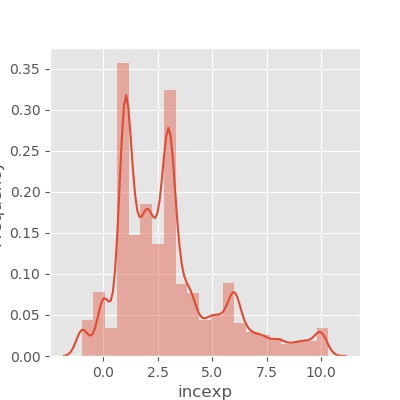
\includegraphics[width=\textwidth]{figures/hist_incexp}
%		\end{subfigure}
%		\begin{subfigure}[b]{0.45\textwidth}
%			\centering
%			\caption{expected growth of real}
%			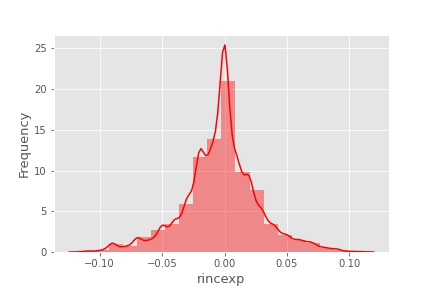
\includegraphics[width=\textwidth]{figures/hist_rincexp}
%		\end{subfigure}
%	\end{figure}
%	\begin{itemize}
%		\item nominal income: right-skewed and mostly positive   
%		\item real income: symmetric around zero  
%	\end{itemize}
%\end{frame}

\begin{frame}{Within-group dispersion in perceived income risks}
	\begin{figure}
		\centering
		\label{rincstd_hist}
%			\begin{subfigure}[b]{0.45\textwidth} 
%			\centering
%			\caption{income risks (nominal)}
%		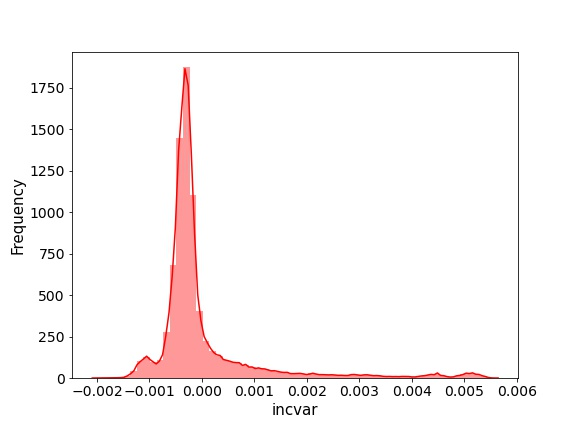
\includegraphics[width=\textwidth]{figures/hist_incvar.jpg}
%		\end{subfigure}
	%	\begin{subfigure}[b]{0.45\textwidth}
%		\centering
%		\caption{income risks}
		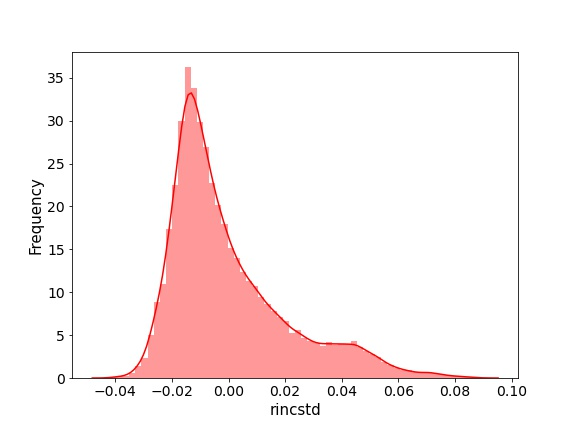
\includegraphics[width=0.6\textwidth]{figures/hist_rincstd.jpg}
%	\end{subfigure}
	\end{figure}
	\begin{itemize}
		\item  residuals controlling for observables/time fixed effects ($R^2=0.07$) 
		\item average PR:  $3.5\%$ in std; 10/90 IQR: $5.2\%$ in std \quad \hyperlink{appendix:incstd}{\beamerbutton{nominal}}  \quad \hyperlink{appendix:incskew}{\beamerbutton{skewness}}    
% \item just a lower bound: before adjustment of unemployment risk 
	\end{itemize}
\end{frame}


\begin{frame}{Perceived risks by annual earning}
	\begin{figure}
		\centering
		\label{boxplot_hhinc}
		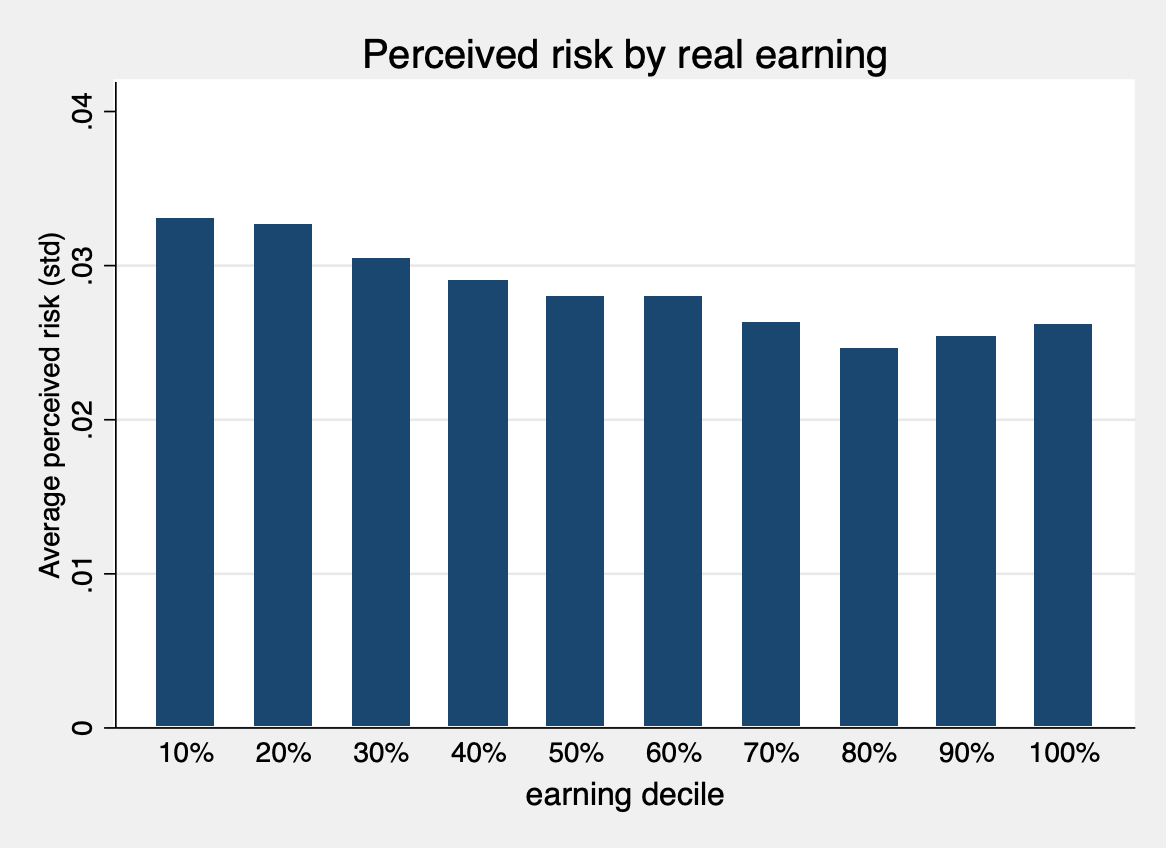
\includegraphics[width=0.7\textwidth]{figures/boxplot_rvar_earning}
	\end{figure}
	%\begin{itemize}
	%\item Similar to the pattern of earning growth dispersion conditional on income in \cite{bloom2018great}. 
	%\end{itemize}
 \end{frame}


\begin{frame}{Monthly earning inequality and volatility}
	\begin{figure}
		\centering
		\label{earning_inequality_volatility}
		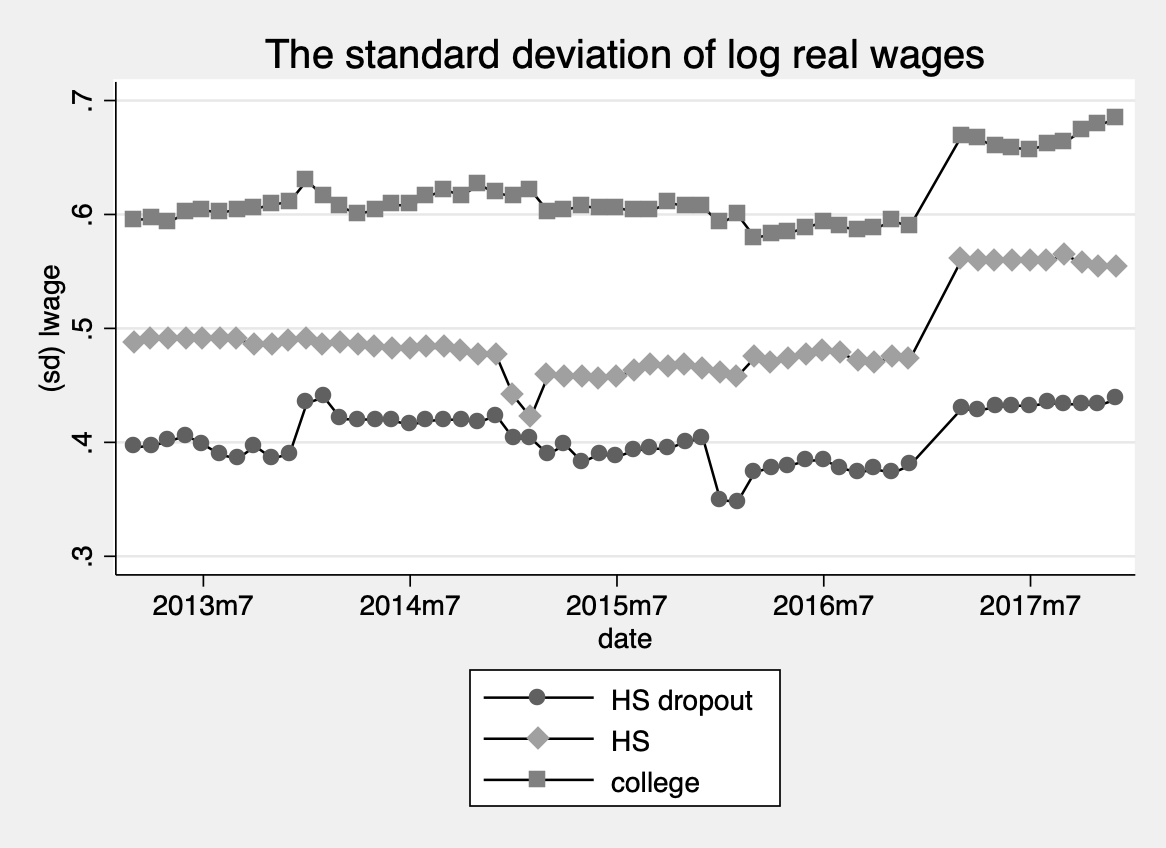
\includegraphics[width=0.45\textwidth]{figures/log_wage_sd_by_edu.png} 
			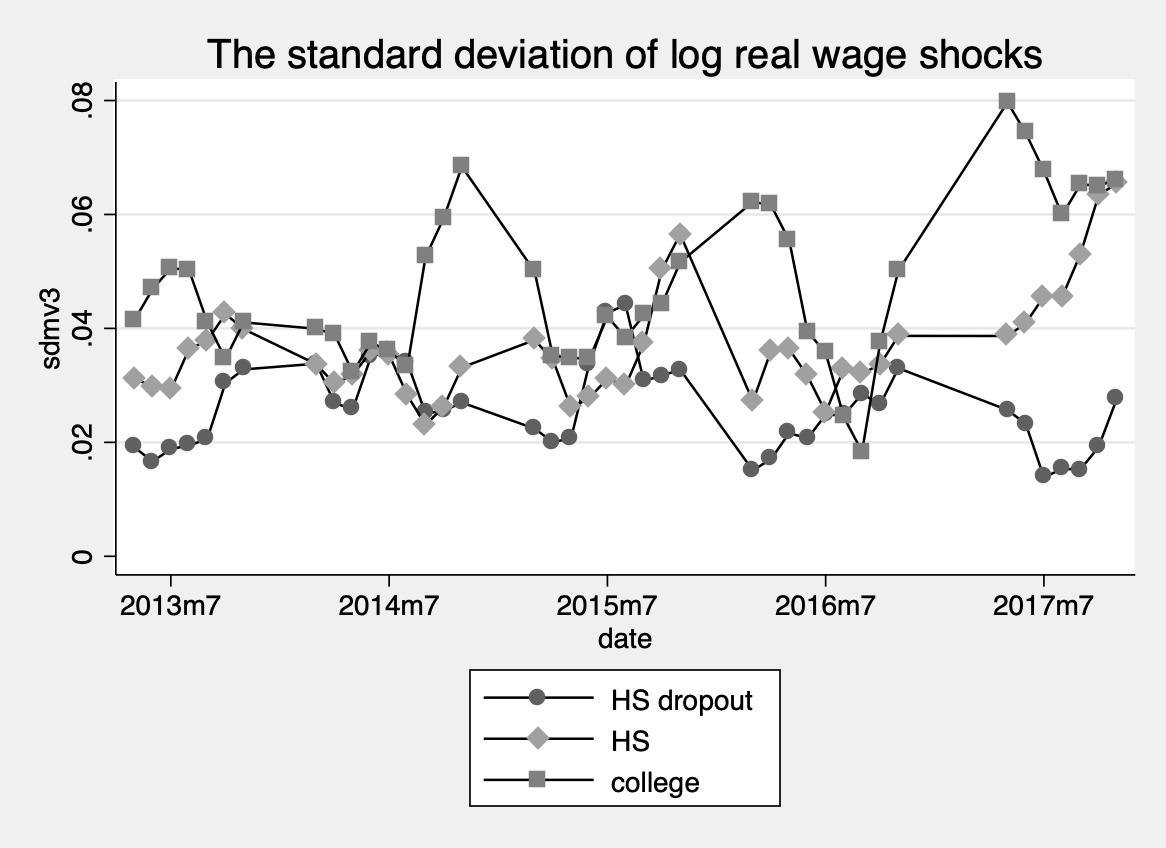
\includegraphics[width=0.45\textwidth]{figures/log_wage_shk_gr_sd_by_edu.png} 
	\end{figure}
	%\begin{itemize}
	%\item Similar to the pattern of earning growth dispersion conditional on income in \cite{bloom2018great}. 
	%\end{itemize}
\end{frame}

\begin{frame}{By \textbf{age}/gender/education}
	\label{age_compare}
	\begin{figure}[ht]
		%\caption{Perceived Risk} 
		\label{compare_by_age_gender_educ}
		\centering
		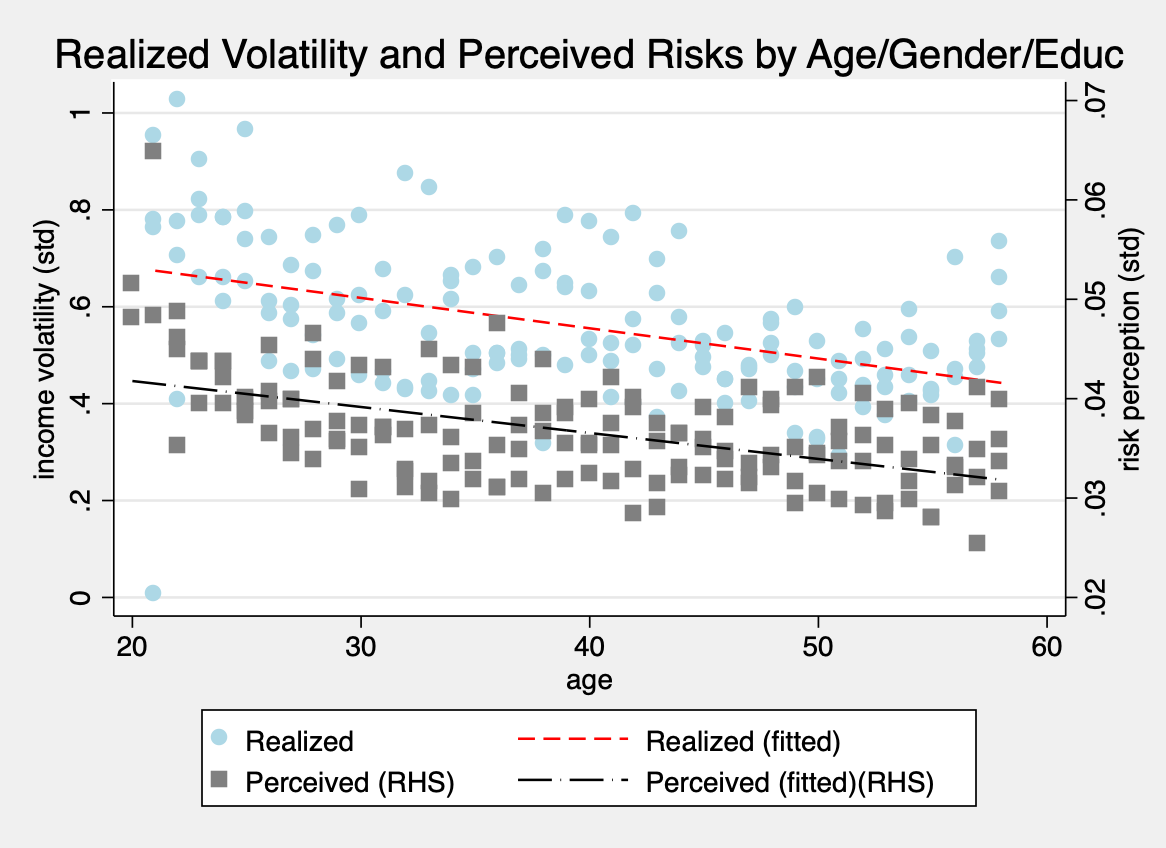
\includegraphics[width=0.60\textwidth]{figures/real_log_wage_shk_gr_by_age_edu_gender_compare.png}
	\end{figure}
\begin{itemize}
	\item e.g. a male high school graduate aged 30   \hyperlink{appendix:age_gender_educ_compare_figure}{\beamerbutton{inequality}} \quad \hyperlink{appendix:age_compare_figure}{\beamerbutton{by age}}  
	\quad  \hyperlink{appendix:age_educ_compare_figure}{\beamerbutton{by age/education}}  
	\quad  \hyperlink{appendix: compare_by_cohort}{\beamerbutton{by 5-yr of birth/education/gender}}  
	\item consistent with  \cite{moffitt2002trends}, \cite{sabelhaus2010great}
	%	\item in line with existing findings, for instance  
	%	\cite{bloom2018great}. 
\end{itemize}
\end{frame}



\begin{frame}{By \textbf{5-yr of birth/age}}
	\label{cohort_age_compare}
	\begin{figure}[ht]
		%\caption{Perceived Risk} 
		\label{compare_by_cohort_age}
		\centering
		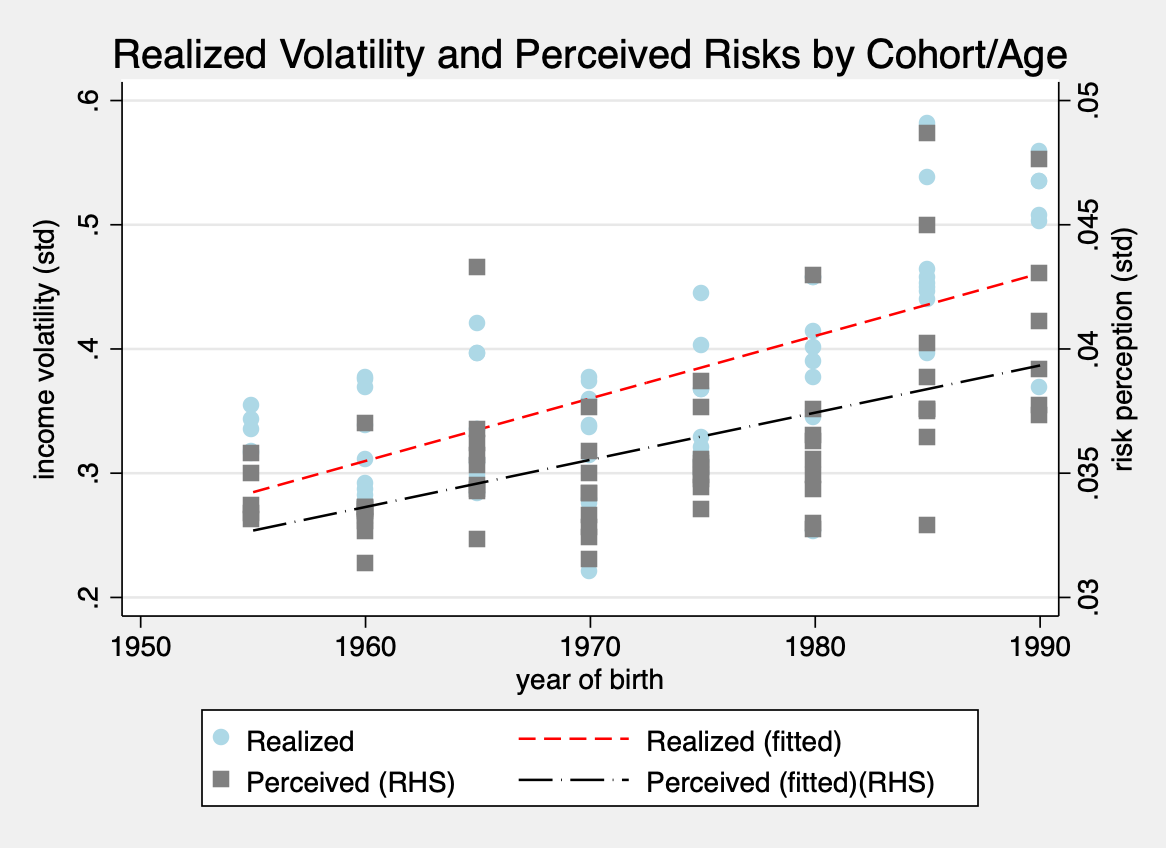
\includegraphics[width=0.65\textwidth]{figures/real_log_wage_shk_gr_by_byear_age_compare.png}
		%	\begin{subfigure}[b]{0.46\textwidth}
		%			\caption{skewness}
		%			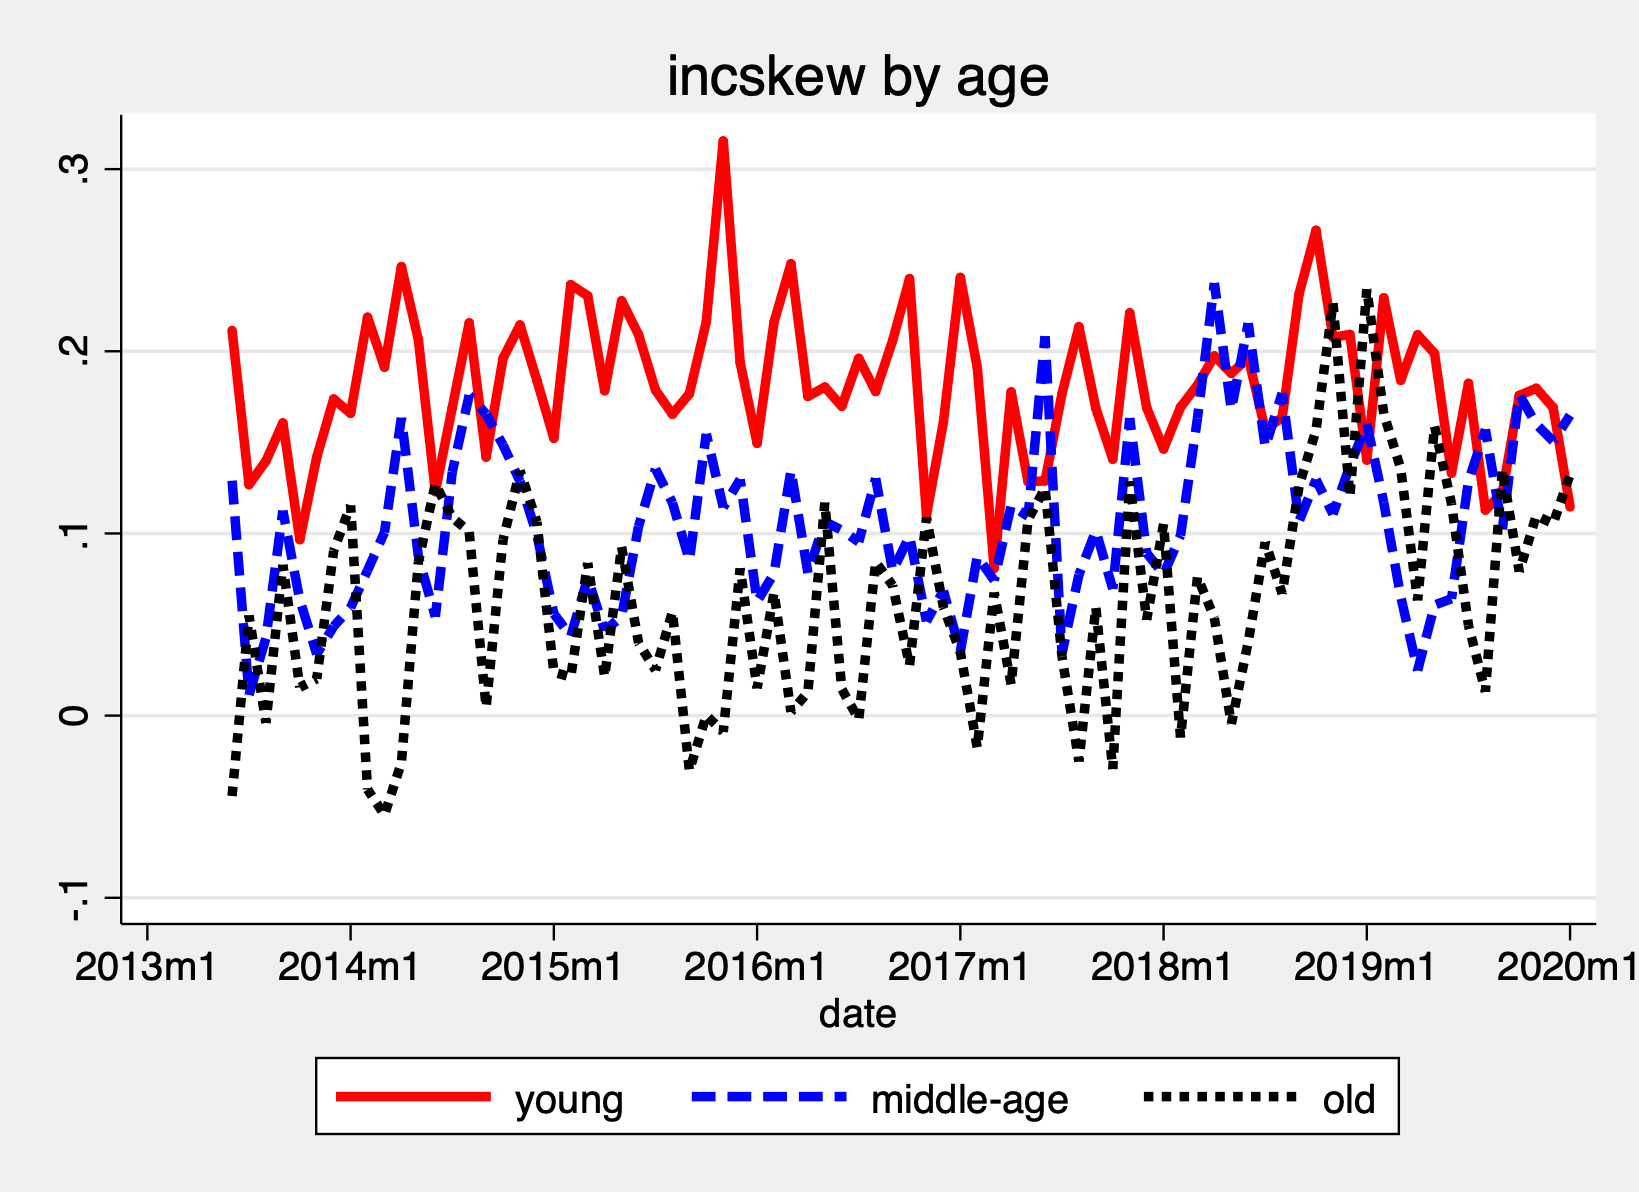
\includegraphics[width=\textwidth, height = 0.33\textheight]{figures/ts_incskew_age_g_mean.png}
		%	\end{subfigure}
	\end{figure}
	\begin{itemize}
		\item e.g. born between 1985-1990 at age 25
		\item only possible for post-2013 sample 
			\quad \hyperlink{appendix:cohort_age_compare}{\beamerbutton{inequality}}     
	\end{itemize}
\end{frame}



\subsection{Permanent versus transitory risks}


\begin{frame}{Time series structure of income shock}

\begin{equation*}
	\begin{split}
& e_{i,c,t} = \underbrace{p_{i,c,t}}_{\text{Ind Permanent}} + \underbrace{\eta_{i,c,t}}_{\text{Ind Transitory}} \\
& p_{i,c,t+1} = p_{i,c,t} + \psi_{i,c,t+1} \\
& \underbrace{\eta_{i,c,t+1}}_{\text{MA(1)}} = \phi \epsilon_{i,c,t} + \epsilon_{i,c,t+1}  
\end{split} 
	\end{equation*}
\begin{itemize}
	\item Different approaches of estimation: 
	\begin{itemize}
		\item approximation: \cite{moffitt2002trends}
		\item variance/covariance matching: \cite{carroll1997nature}, \cite{meghir2004income},  \cite{blundell_consumption_2008}
		\item continuous time: immune to time aggregation: \cite{crawley_search_2019} 
	\end{itemize}
\end{itemize}
\end{frame}



\begin{frame}{Permanent versus transitory risks}
	\label{cohort_age_component_compare}
	\begin{figure}[ht]
		%\caption{Perceived Risk} 
		\centering
			\begin{subfigure}[b]{0.44\textwidth}
			\caption{permanent}
		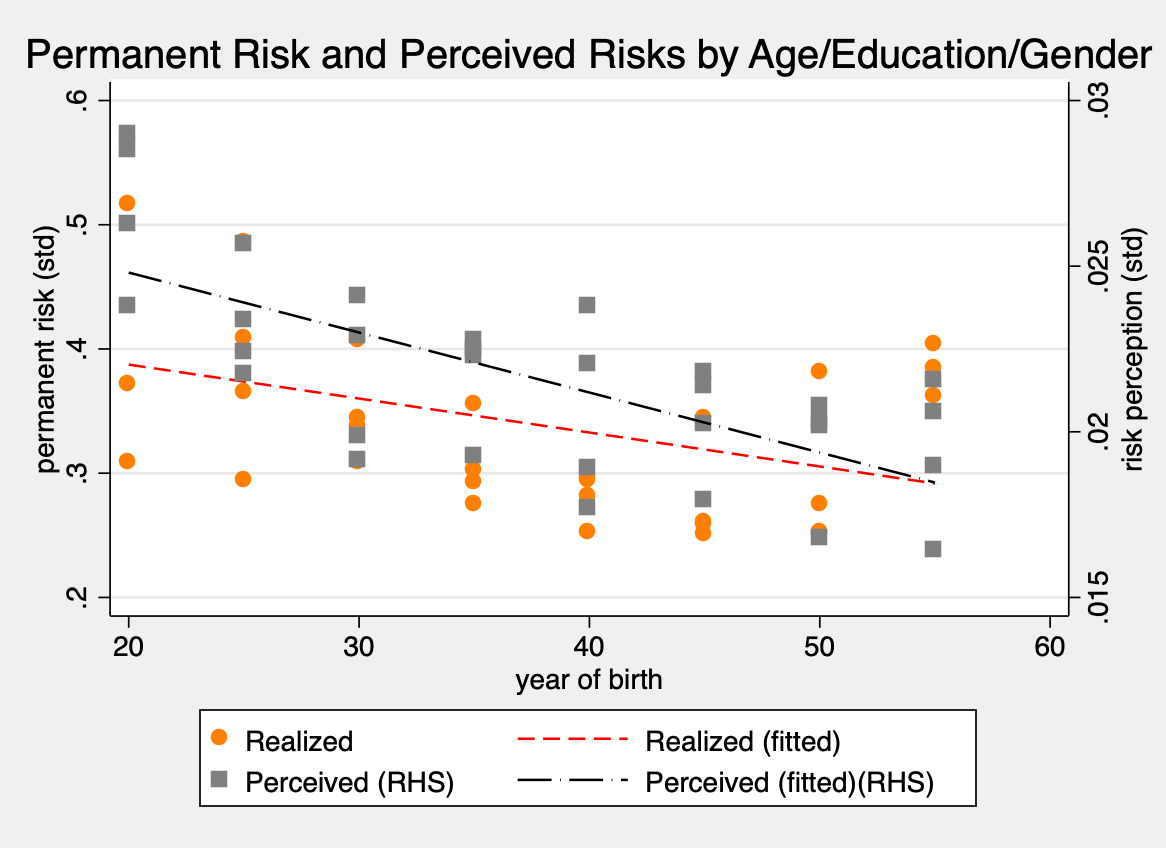
\includegraphics[width=\textwidth]{figures/log_wage_pshk_by_age_5yr_edu_gender_compare.png}
			\end{subfigure}
			\begin{subfigure}[b]{0.44\textwidth}
					\caption{transitory}
					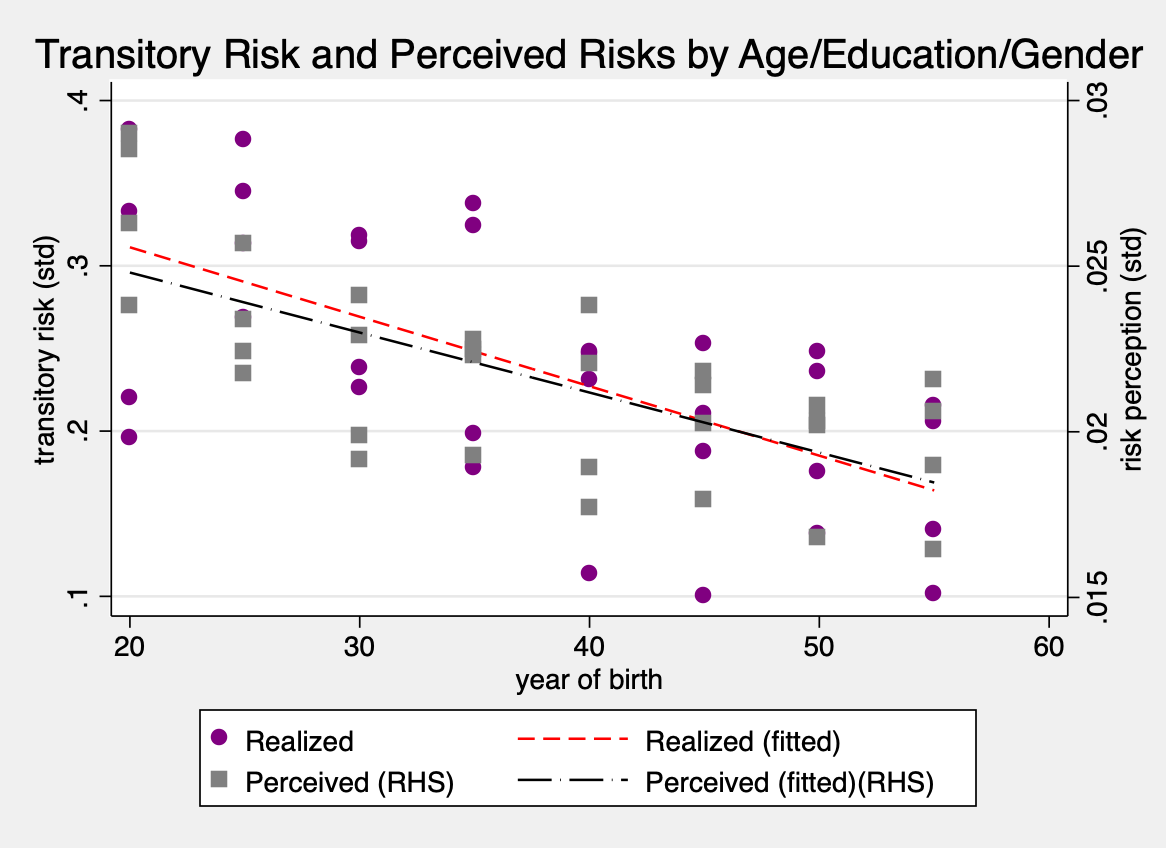
\includegraphics[width=\textwidth]{figures/log_wage_tshk_by_age_5yr_edu_gender_compare.png}
			\end{subfigure} 
	\end{figure}
	\begin{itemize}
		\item e.g. a female high school graduate aged 30-35
		\quad  \hyperlink{appendix:cohort_age_component_compare}{\beamerbutton{5-yr cohort/education/gender}}  
	\end{itemize}
\end{frame}



\begin{frame}{Permanent versus transitory risks (monthly from SIPP)}
	\label{monthly_decomposition_compare}
	\begin{figure}[ht]
		\centering
		\begin{subfigure}[b]{0.44\textwidth}
			\caption{permanent}
			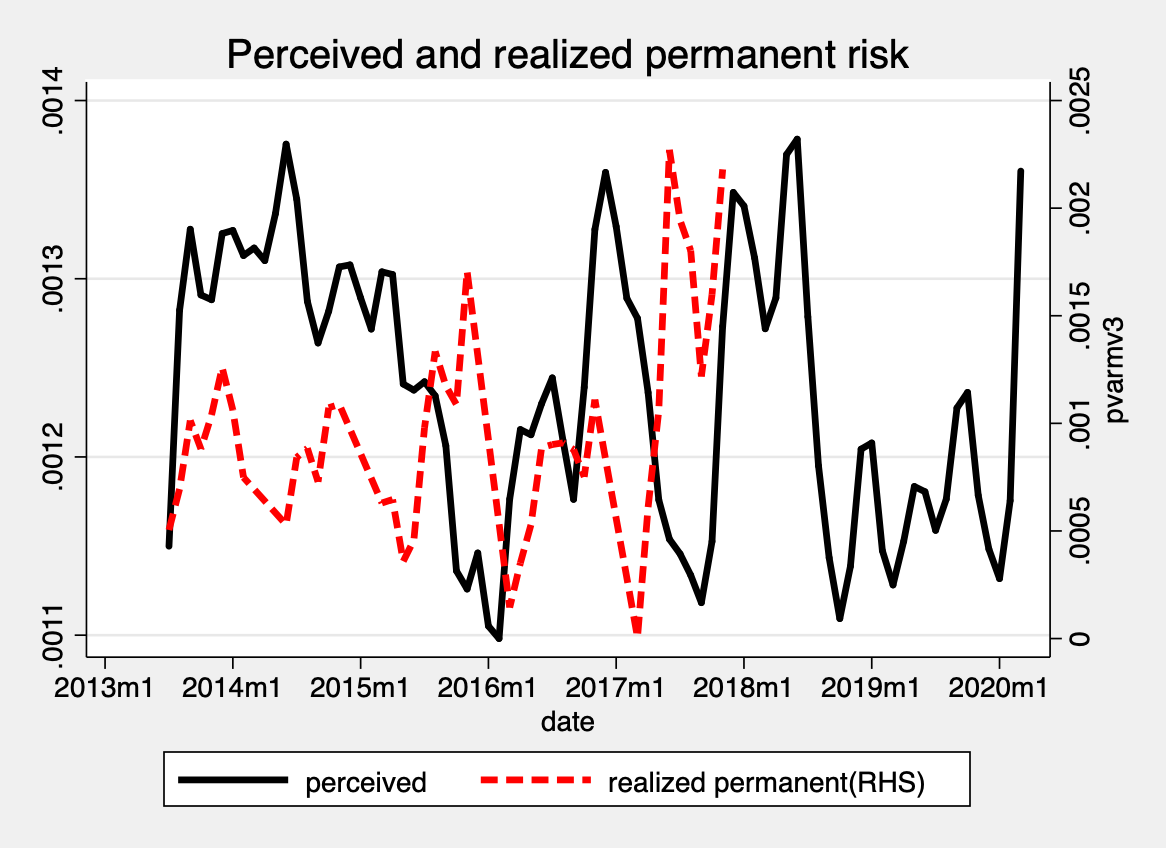
\includegraphics[width=\textwidth]{figures/real_permanent_compare.png}
		\end{subfigure}
		\begin{subfigure}[b]{0.44\textwidth}
			\caption{transitory}
			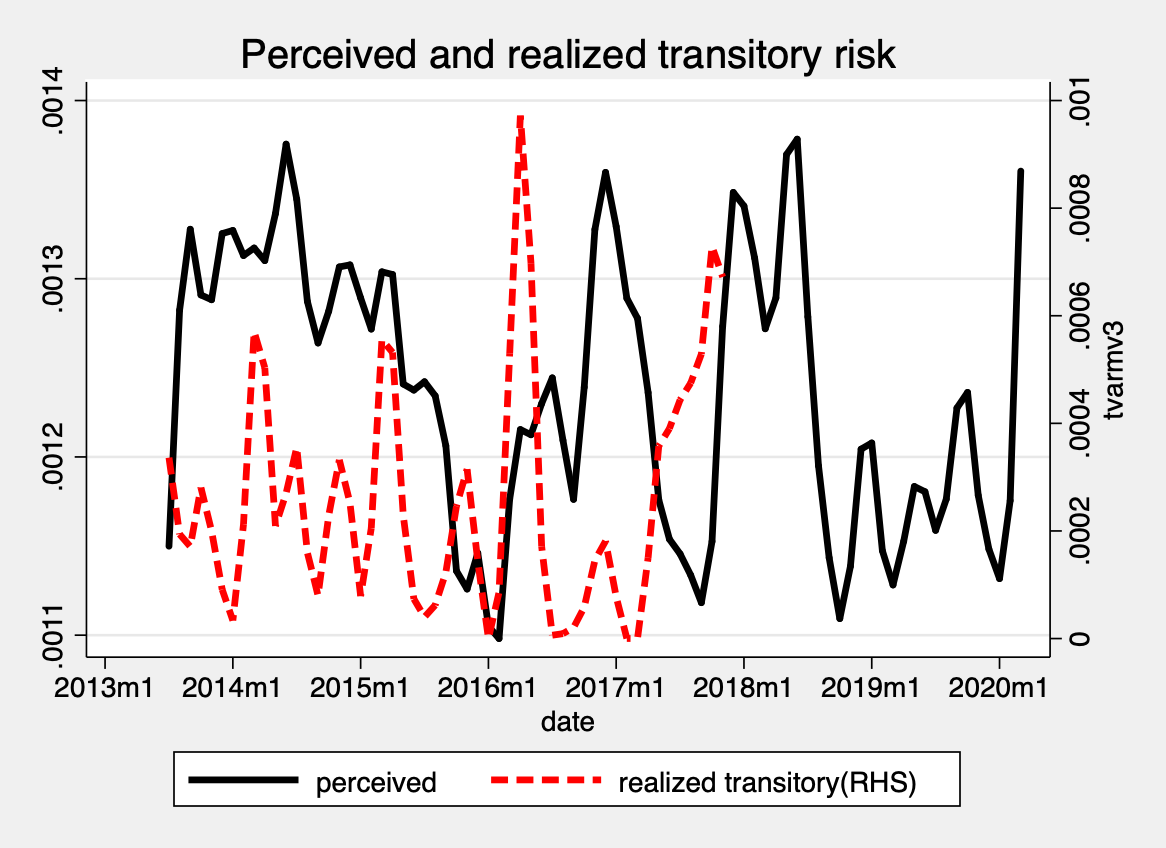
\includegraphics[width=\textwidth]{figures/real_transitory_compare.png}
		\end{subfigure} 
	\end{figure}
	\begin{itemize}
		\item estimated monthly risks (to be aggregated into yearly)
	\end{itemize}
\end{frame}

\subsection{Perceived risks and macroeconomic history}

%% since income risks may difer over time or stochastic,  so the level of risks are not comparable directly between two non-overlapping periods. % therefore, we can treat the income volatility in the past as experiences and examine if it affects risk perceptions. Here we differ from the earlier exercise in that we do not assume the risks are cohort specific. Instead, we just assume the information set, namely the experienced volatility and inequality are different.

% we find the experienced volatility is not correlated with risk perceptions over the past. But experienced inequality is positively correlated with the risk perceptions. 
% furthermore, the average economy has negative impacts on the risk perceptions as well. 


\begin{frame}{Experienced income volatility and perceived risks}
	\begin{figure}
		\centering 
		\label{experience_var_var_var}
		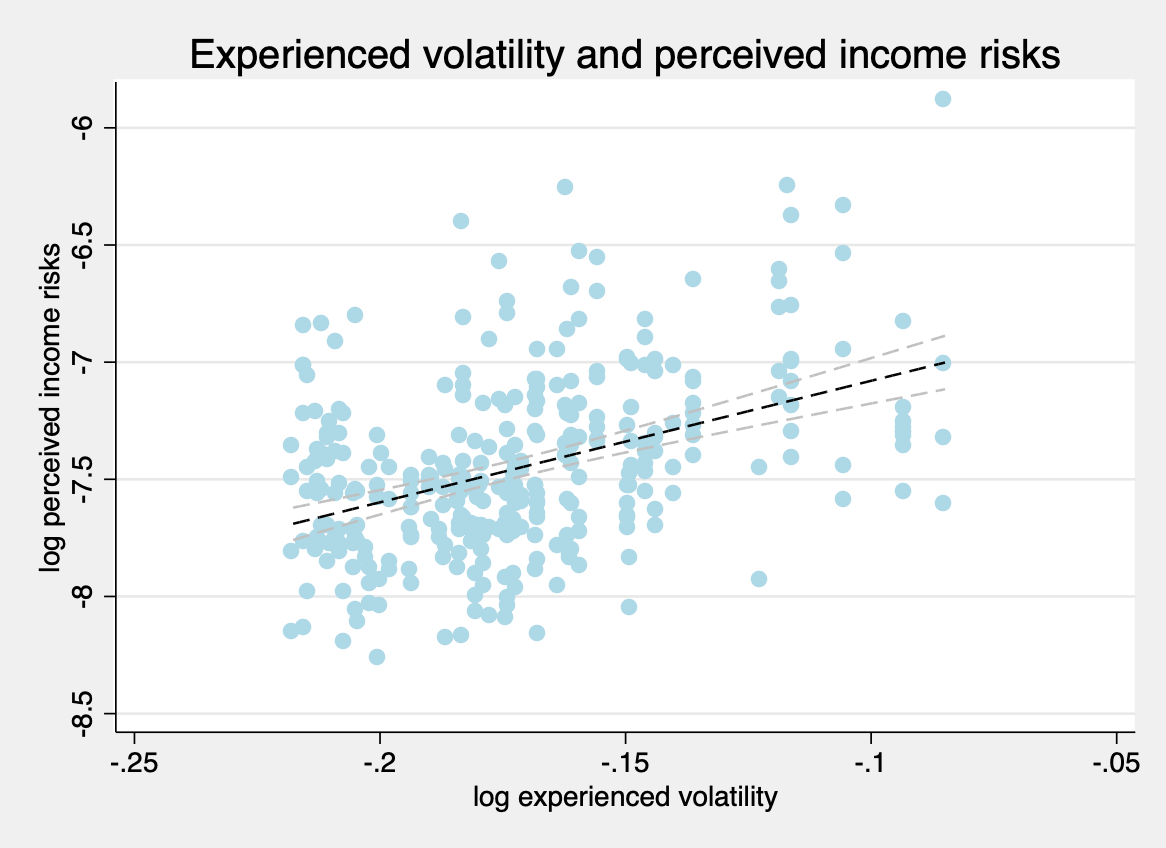
\includegraphics[width=0.6\textwidth]{figures/experience_var_var_data.png}
	\end{figure}
	\begin{itemize}
		\item income volatility conditional on macroeconomic history \cite{storesletten2004cyclical}
		\item e.g. the experience by a 25-year old till 2015 is between 1990-2015
	\end{itemize}
\end{frame}

\begin{frame}{Experienced labor market and perceived risks}
		\begin{figure}
				\centering 
				\label{experience_ue_var}
				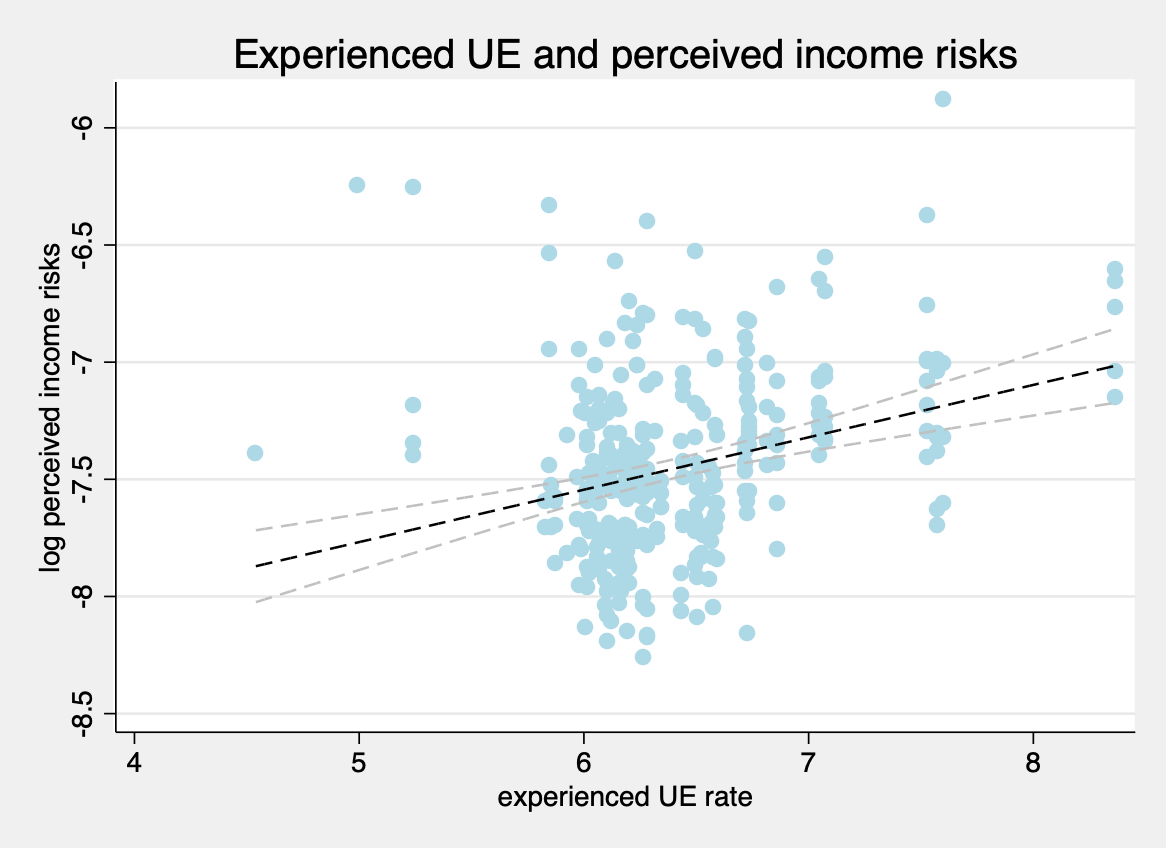
\includegraphics[width=0.6\textwidth]{figures/experience_ue_var_data.png}
			\end{figure}
	\begin{itemize}
		\item e.g. experienced UE by a 25-year old in 2015 is between UE over 1990-2015

	\end{itemize}
\end{frame}


\subsection{Couter-cyclical perceived risks}


\begin{frame}{Perceived risks and recent (past) wage growth}
\label{tsMean3mvrvar_he}
	\begin{itemize}
		\item $\overline{\text{var}_{t}} $: average perceived risk across individuals
		\item  $log(\text{wage}_t) - log(\text{wage}_{t-1/4})$: quarterly growth in average hourly wage
	\end{itemize}
	\begin{figure}
		\centering
		\label{ts_var}
		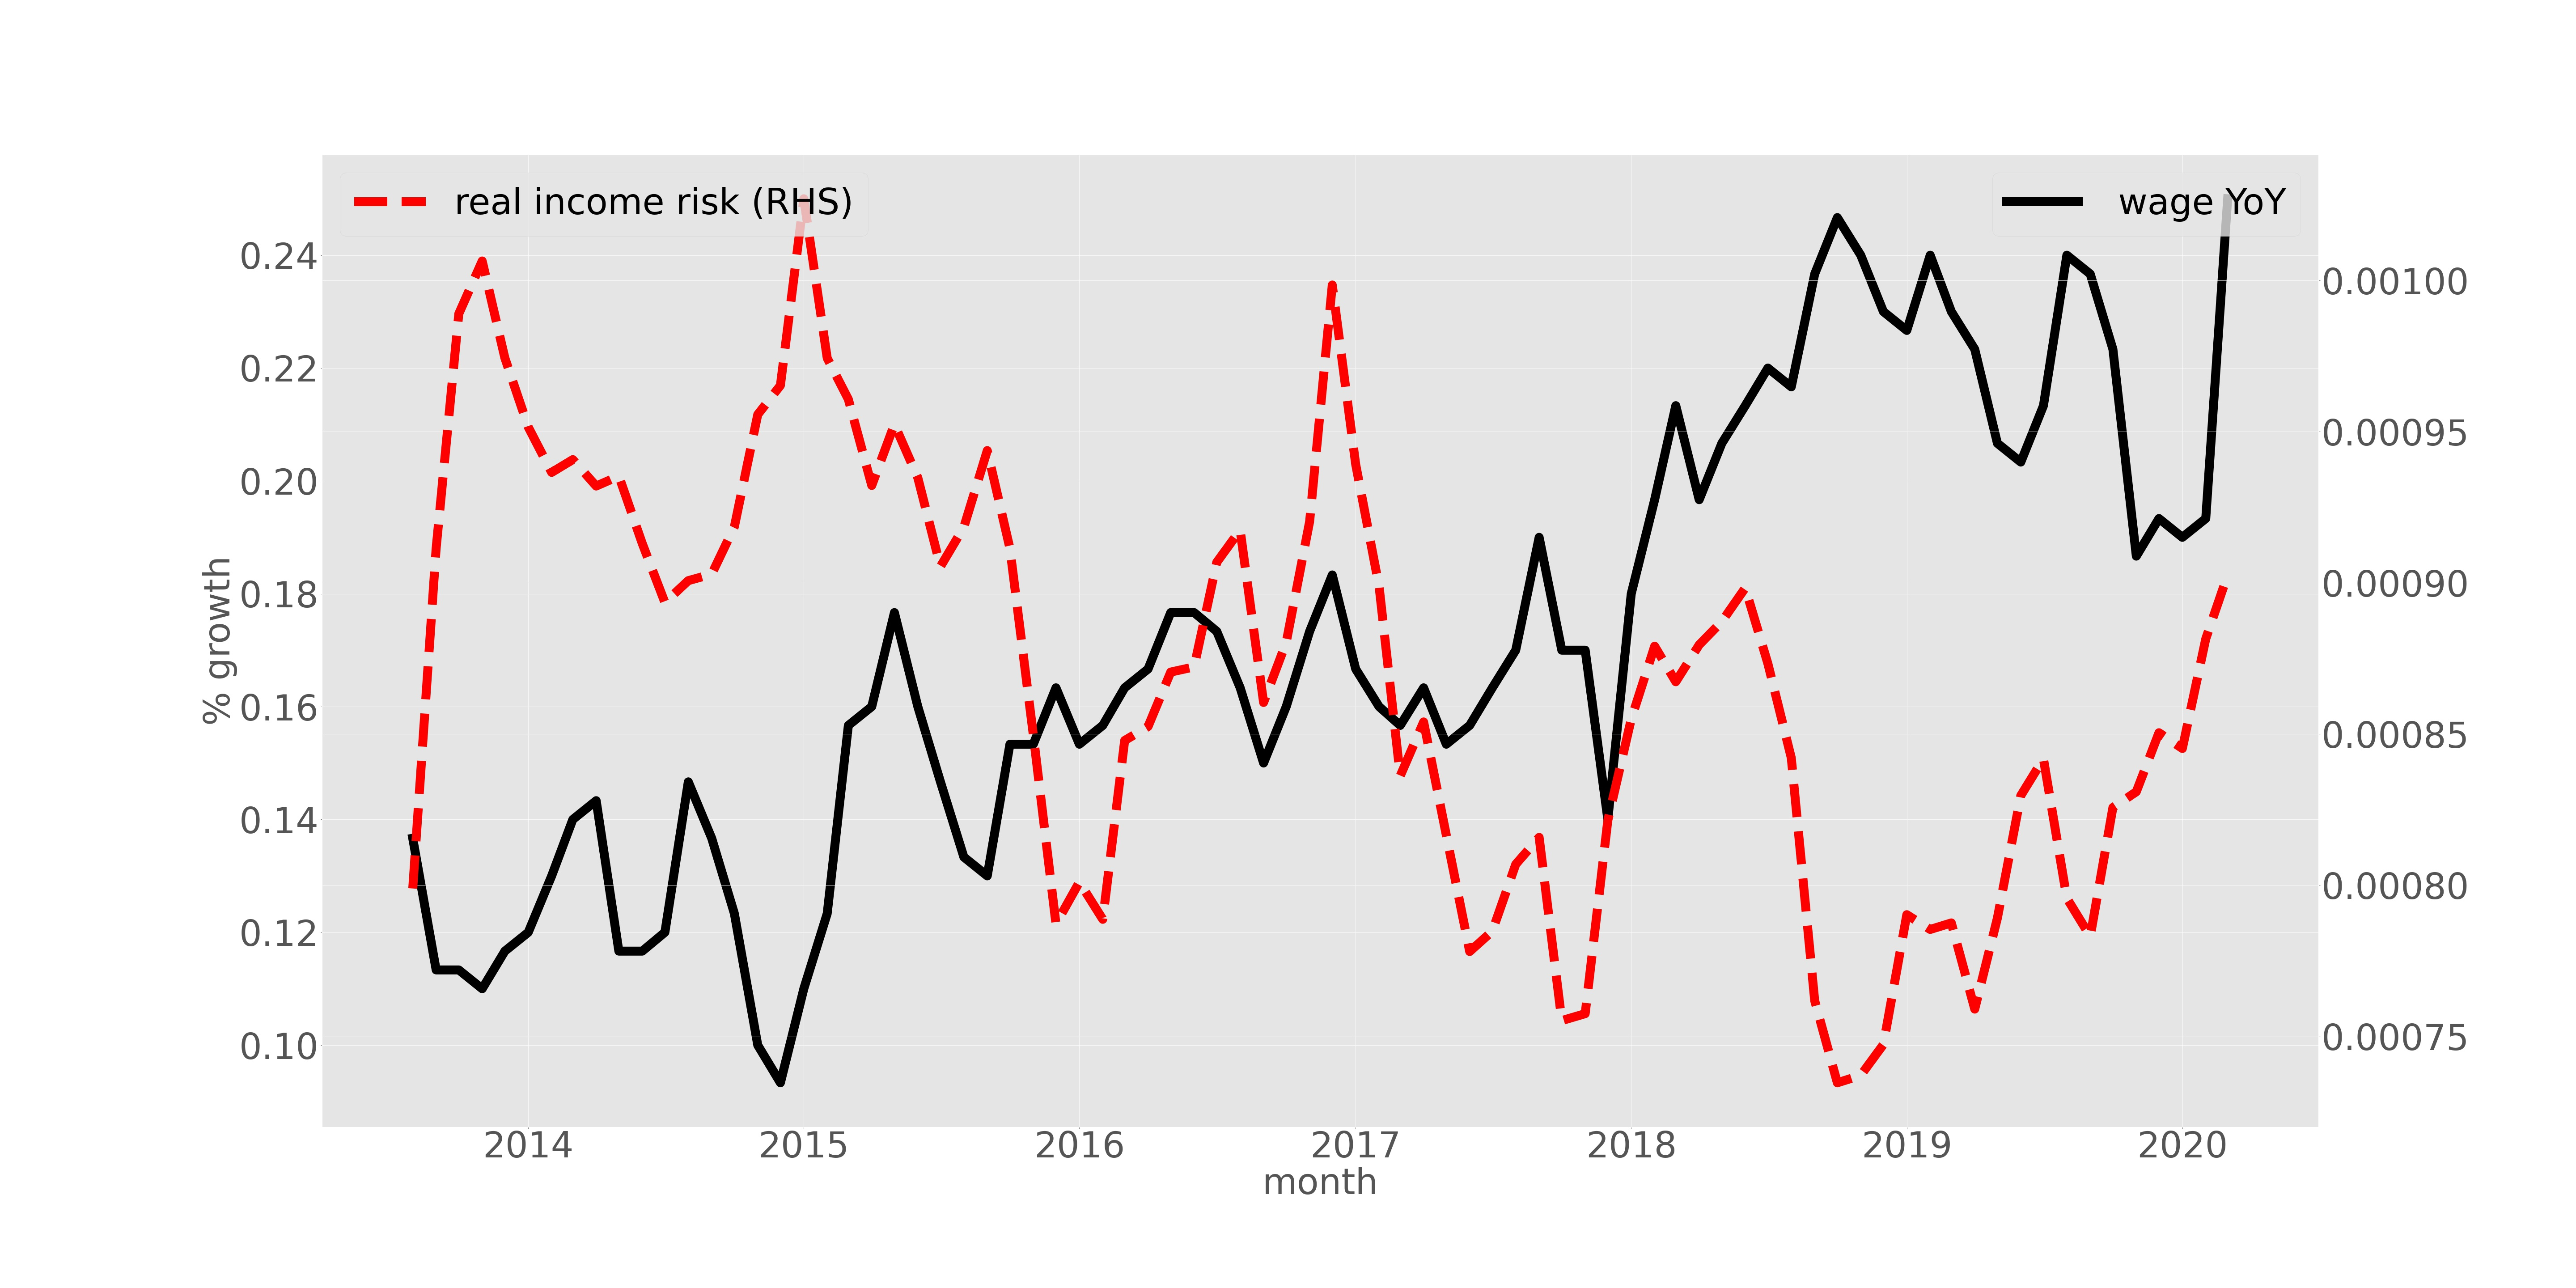
\includegraphics[width=\textwidth]{figures/tsMean3mvrvar_he.jpg}
	\end{figure}
	\quad  \hyperlink{appendix:tsMean3mvrexp_he}{\beamerbutton{expected growth}} 
\end{frame}


%\begin{frame}{Perceived \textcolor{blue}{real} income risks and past wage growth}
%	\begin{itemize}
%	\item $\overline{\text{rvar}_{t}} $
%	\item  $log(\text{wage}_t) - log(\text{wage}_{t-3})$
%\end{itemize}
%	\begin{figure}
%		\centering 
%		\label{ts_skew}
%		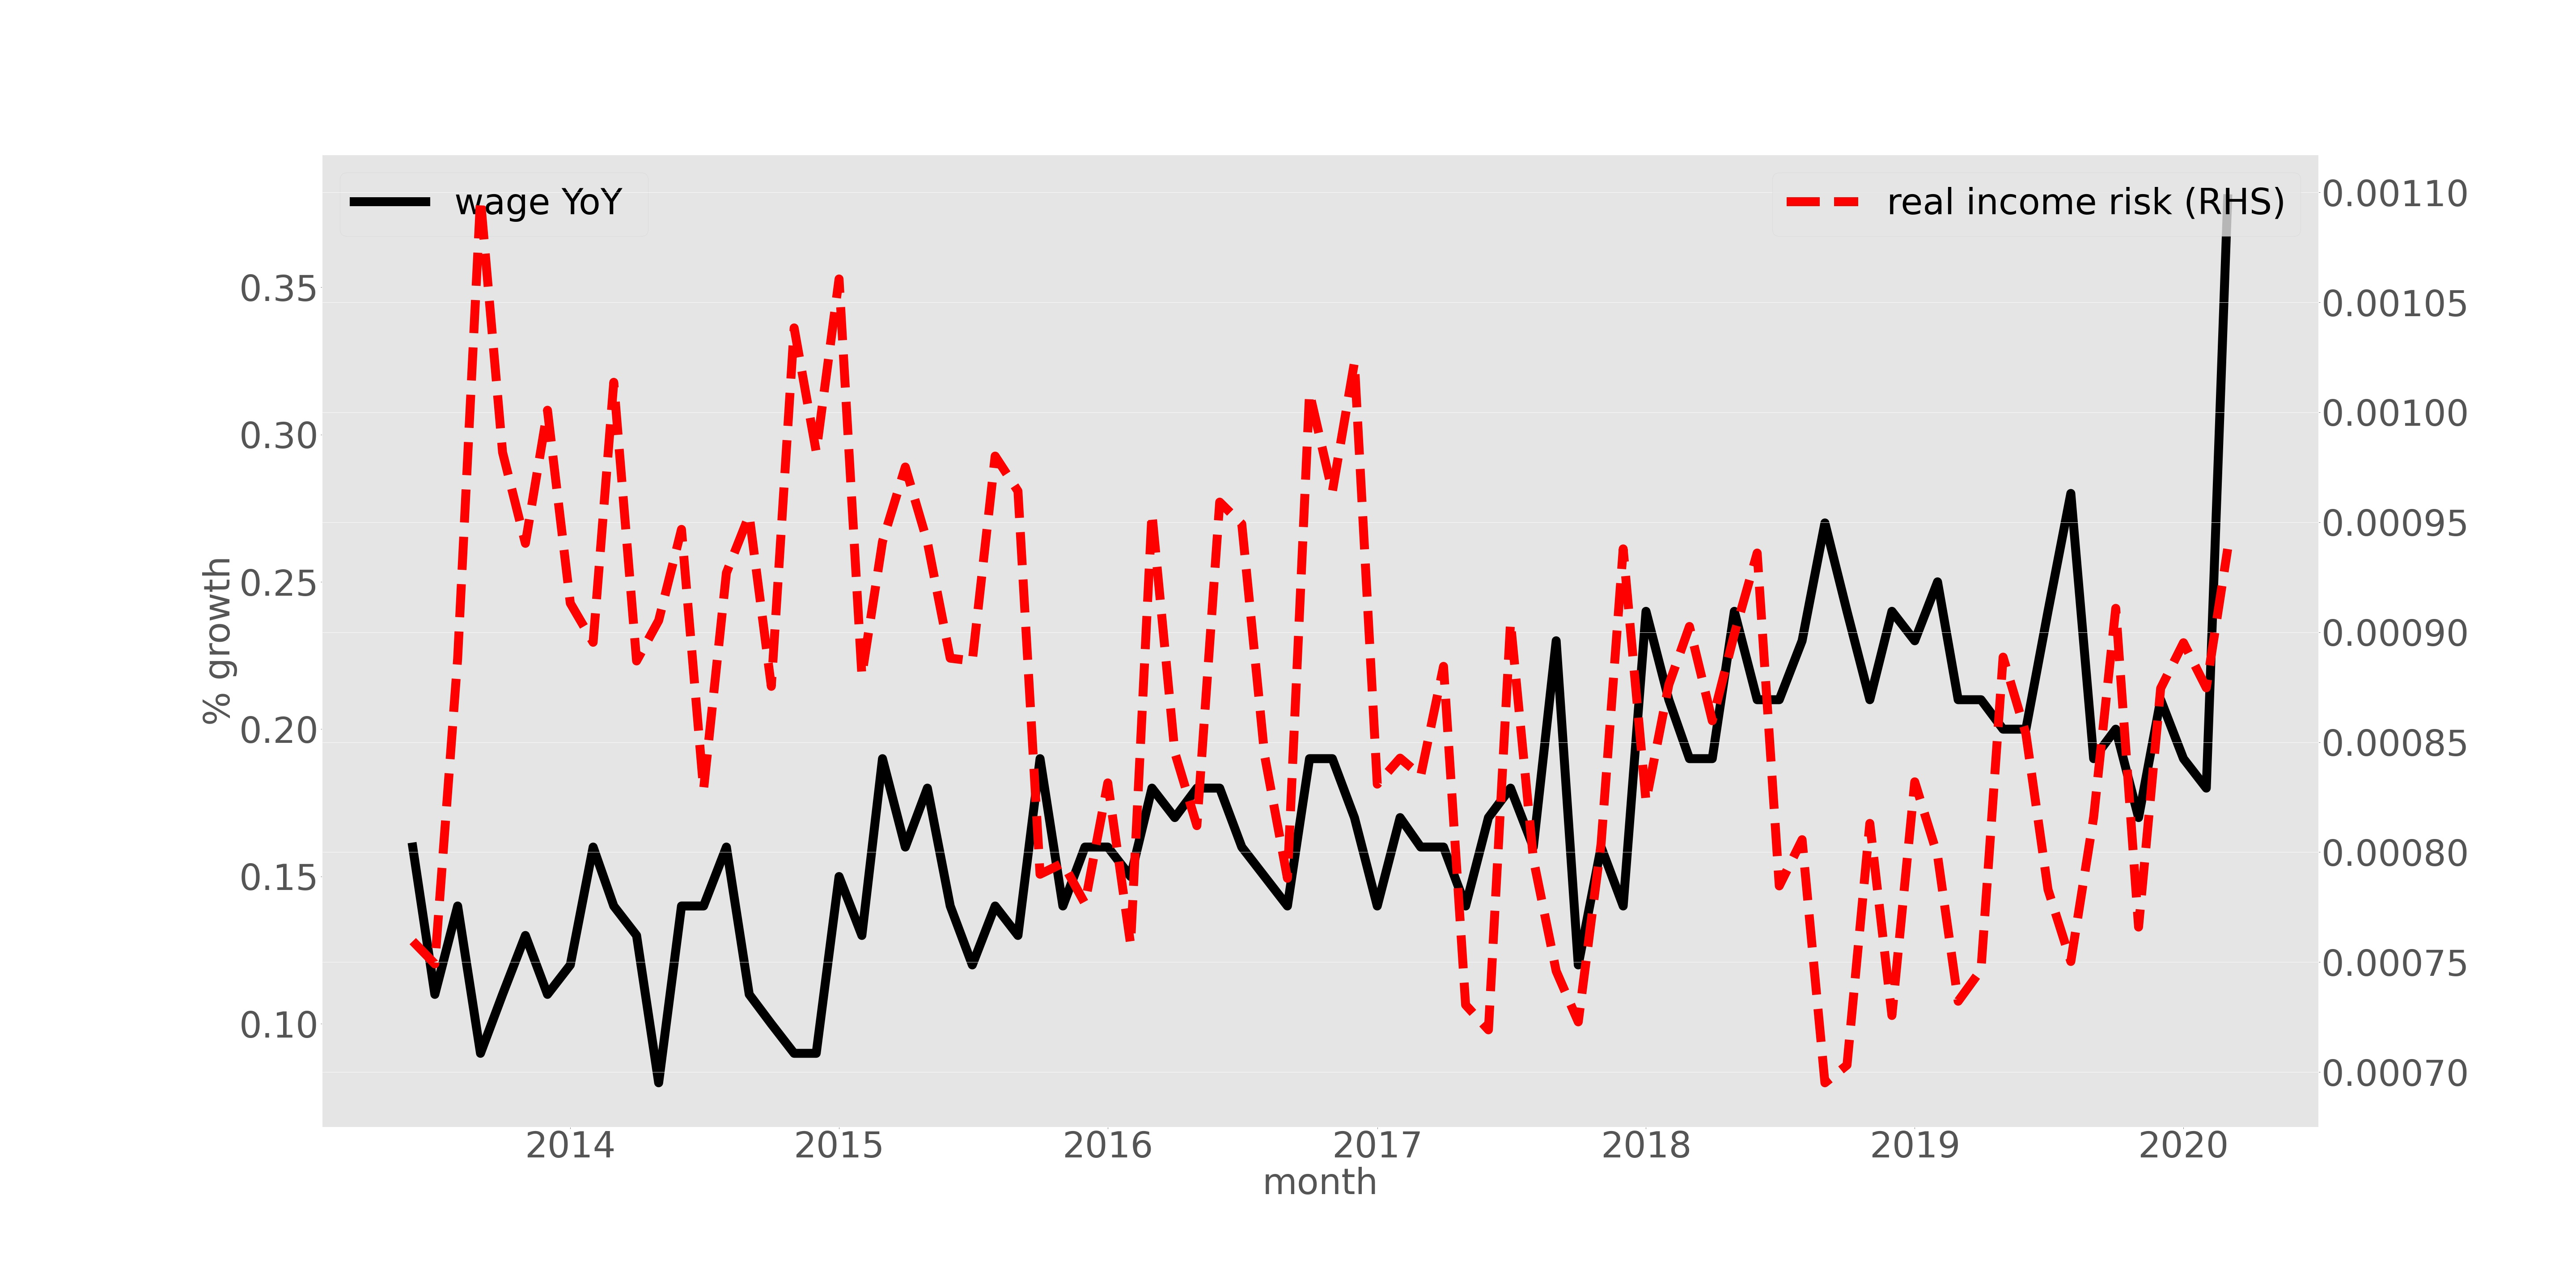
\includegraphics[width=\textwidth]{figures/tsMeanrvar_he.jpg}
%	\end{figure}
%\end{frame}



\begin{frame}{Perceived risks and current labor market condition}
	\begin{eqnarray*}
		\underbrace{\overline{\text{risk}_{t}}}_{\text{average perceived risk}} = \alpha + \textcolor{red}{\beta} \underbrace{(log(\text{wage}_{t-k/12}) - log(\text{wage}_{t-(k-3)/12}))}  _{\text{wage growth}}  + \epsilon_{i,t}	 \\
		\quad \forall k =0...4
	\end{eqnarray*}
	
	\begin{table}
		\centering
		%\caption{Correlation between Perceived Income Risks and Stock Market Return}
		\label{macro_corr_he}
		\adjustbox{max height=0.5\textheight, max width=\textwidth}{ 
		\begin{tabular}{lllll}
				\hline 
			& mean:var & mean:iqr & mean:rvar & mean:skew \\
				\hline 
			0 & -0.28**  & -0.42*** & -0.48***  & -0.02     \\
			1 & -0.42*** & -0.53*** & -0.51***  & 0.12      \\
			2 & -0.43*** & -0.48*** & -0.44***  & -0.01     \\
			3 & -0.43*** & -0.48*** & -0.42***  & -0.1      \\
			4 & -0.31*** & -0.41*** & -0.32***  & -0.21*   \\
			\hline 
		\end{tabular}
		}
	\end{table}
\begin{itemize}
	\item Counter-cyclical income risks: \cite{storesletten2004cyclical}, \cite{guvenen2014nature}, \cite{bayer2019precautionary}
	%\item Counter-cyclical skewness: \cite{guvenen_empirical_2009}, \cite{guvenen_inferring_2014} 
\end{itemize}
\end{frame}



\begin{frame}{Perceived risks and current labor market condition}
	\begin{eqnarray*}
		\underbrace{\overline{\text{risk}_{s,t}} }_{\text{median perceived risk in state $s$}}= r + \textcolor{red}{\psi} \underbrace{LM_{s,t}}_{\text{state labor market condition}}  + \eta_{s,t}
	\end{eqnarray*}
	\begin{table}
		\centering
		%\caption{Correlation between Perceived Income Risks and Stock Market Return}
		\label{macro_corr_he_state}
		\adjustbox{max height=0.5\textheight, max width=\textwidth}{ 
			\begin{tabular}{lllll}
				\hline 
				& (1)                & (2)                & (3)               & (4)               \\
				\hline 
				& log(var) & log(risk) & log(iqr) & log(iqr) \\
				\hline 
				wage growth & -0.05***           &                    & -0.03***          &                   \\
				
				& (0.01)             &                    & (0.01)            &                   \\
				unemp rate &                    & 0.04*              &                   & 0.04***           \\
				&                    & (0.02)             &                   & (0.01)            \\
				\hline 
				Observations      & 3529               & 3529               & 3546              & 3546              \\
				R-squared         & 0.023              & 0.020              & 0.025             & 0.028            \\
				\hline 
			\end{tabular}
		}
	\end{table}
\end{frame}

\subsection{Perceived unemployment risks}



\begin{frame}{Perceived unemployment risk and realized job seperation rate}
	\begin{figure}
		\centering
		\label{ue_expectations}
		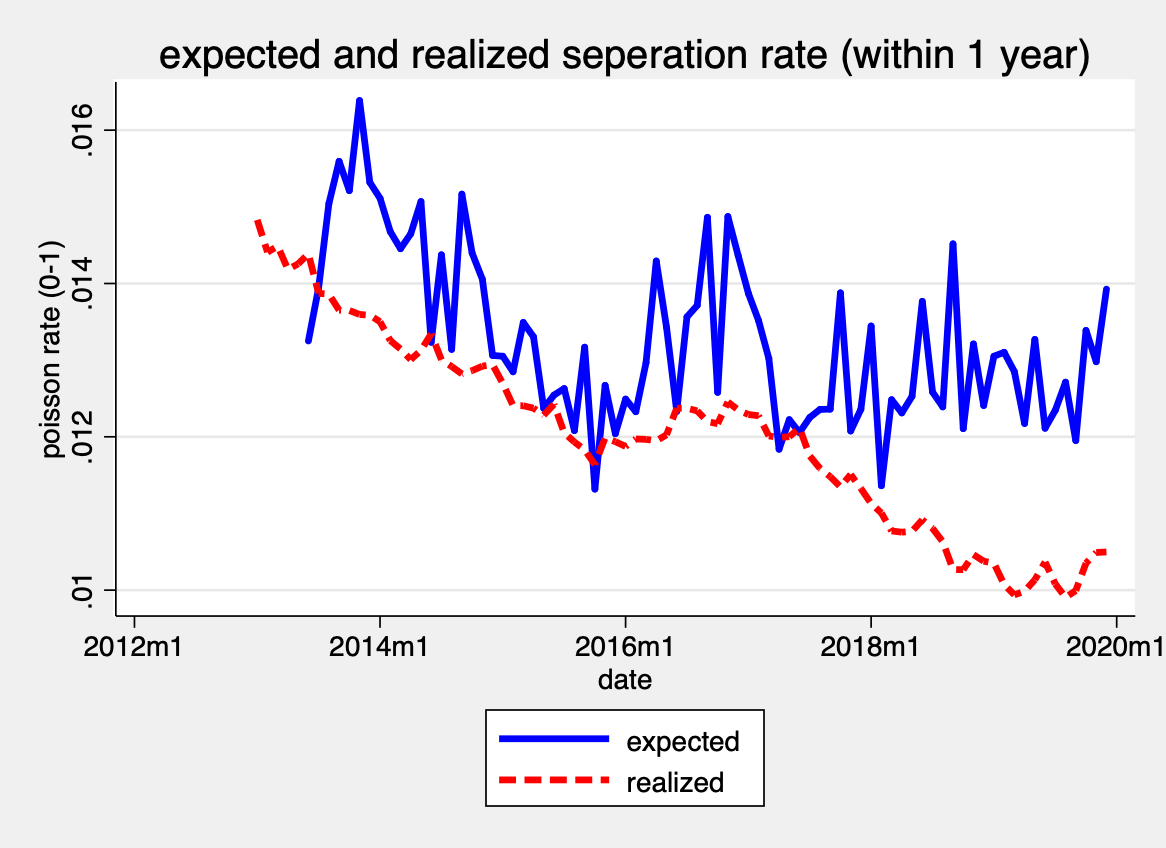
\includegraphics[width=0.7\textwidth]{figures/seperation_rate_1y}
	\end{figure}
	\begin{itemize}
	\item realized job separation rate is computed from CPS survey 
	\end{itemize}
\end{frame}


\subsection{Extrapolation of recent experience}

\begin{frame}{Extrapolaton from \textcolor{blue}{individual} risk perceptions}
	
	\begin{itemize}
		\item experienced volatility $\rightarrow$ PR
		\item recent unemp experience $\rightarrow$ PR
	\end{itemize}
\begin{table}
	\centering
	\label{extrapolation}
	\adjustbox{max height=0.5\textheight, max width=\textwidth}{ 
	\begin{tabular}{lllllllllll}
		\hline 
		& (1)       & (2)       & (3)       & (4)       & (5)        & (6)        & (7)        & (8)        & (9)        & (10)       \\
		\hline 
		income shock squared                  & 0.0225*** & 0.0222*** & 0.0217*** & 0.0207*** & 0.000773   & 0.00205*** & 0.000566   & 0.00183*** & 0.000614   & 0.00184*** \\
		& (0.00562) & (0.00570) & (0.00562) & (0.00564) & (0.000743) & (0.000516) & (0.000744) & (0.000515) & (0.000745) & (0.000516) \\
		&           &           &           &           &            &            &            &            &            &            \\
		recently unemployed                   &           &           &           & 0.511*    & 0.228***   & 0.0895***  &            &            &            &            \\
		&           &           &           & (0.260)   & (0.0330)   & (0.0200)   &            &            &            &            \\
		&           &           &           &           &            &            &            &            &            &            \\
		unemployed since m-8&           &           &           &           &            &            & 0.161***   & 0.0783***  &            &            \\
		&           &           &           &           &            &            & (0.0207)   & (0.0121)   &            &            \\
		&           &           &           &           &            &            &            &            &            &            \\
		unemployed since y-1&           &           &           &           &            &            &            &            & 0.138***   & 0.0701***  \\
		&           &           &           &           &            &            &            &            & (0.0193)   & (0.0113)   \\
		Observations                          & 3662      & 3662      & 3662      & 3662      & 3701       & 1871       & 3701       & 1871       & 3701       & 1871       \\
		R-squared                             & 0.004     & 0.013     & 0.016     & 0.017     & 0.015      & 0.030      & 0.019      & 0.041      & 0.016      & 0.039      \\
		\hline 
	\end{tabular}
}
\end{table}
\end{frame}



\subsection{Perceived risks and decisions}


\begin{frame}{Perceived risks and household spending}
	
	\begin{eqnarray*}
		E_{i,t} (\Delta c_{i,t+1}) = u_0 + \textcolor{red}{u_1} \overline{\text{risks}}_{i,t} (\Delta y_{i,t+1}) + \xi_{i,t}  
	\end{eqnarray*}
	\begin{table}
		\centering
		%\caption{Perceived income risks and household spending}
		\label{spending_reg}
		\adjustbox{max height=0.5\textheight, max width=\textwidth}{ 
			
\begin{tabular}{lllllll}
	\hline 
	& (1)      & (2)      & (3)      & (4)      & (5)      & (6)      \\
		\hline 
	perceived earning risk           & 8.394*** & 8.399*** & 3.642*** & 3.243*** &          &          \\
	& (1.175)  & (1.176)  & (0.533)  & (0.537)  &          &          \\
	&          &          &          &          &          &          \\
	perceived earning risk (nominal) &          &          &          &          & 3.656*** &          \\
	&          &          &          &          & (0.990)  &          \\
	&          &          &          &          &          &          \\
	perceived ue risk                &          &          &          &          &          & 0.353*** \\
	&          &          &          &          &          & (0.0553) \\
		\hline 
	R-squared                        & 0.0010 & 0.00282  & 0.928    & 0.928    & 0.941    & 0.633    \\
	Sample Size                      & 53178    & 53178    & 53178    & 53178    & 54584    & 6269     \\
	Time FE                          & No       & Yes      & No       & Yes      & Yes      & No       \\
	Individual FE                    & No       & No       & Yes      & Yes      & Yes      & Yes     \\
		\hline 
\end{tabular}
		}
	\end{table}
	\begin{itemize}
		\item  Higher perceived risks $\rightarrow$ higher expected spending growth. 
	\end{itemize}
\end{frame}

%\begin{frame}{\textcolor{red}{Counter-cyclical} perceived risks, continued}
%		\begin{figure}
%		\centering 
%		\label{var_experience_var}
%		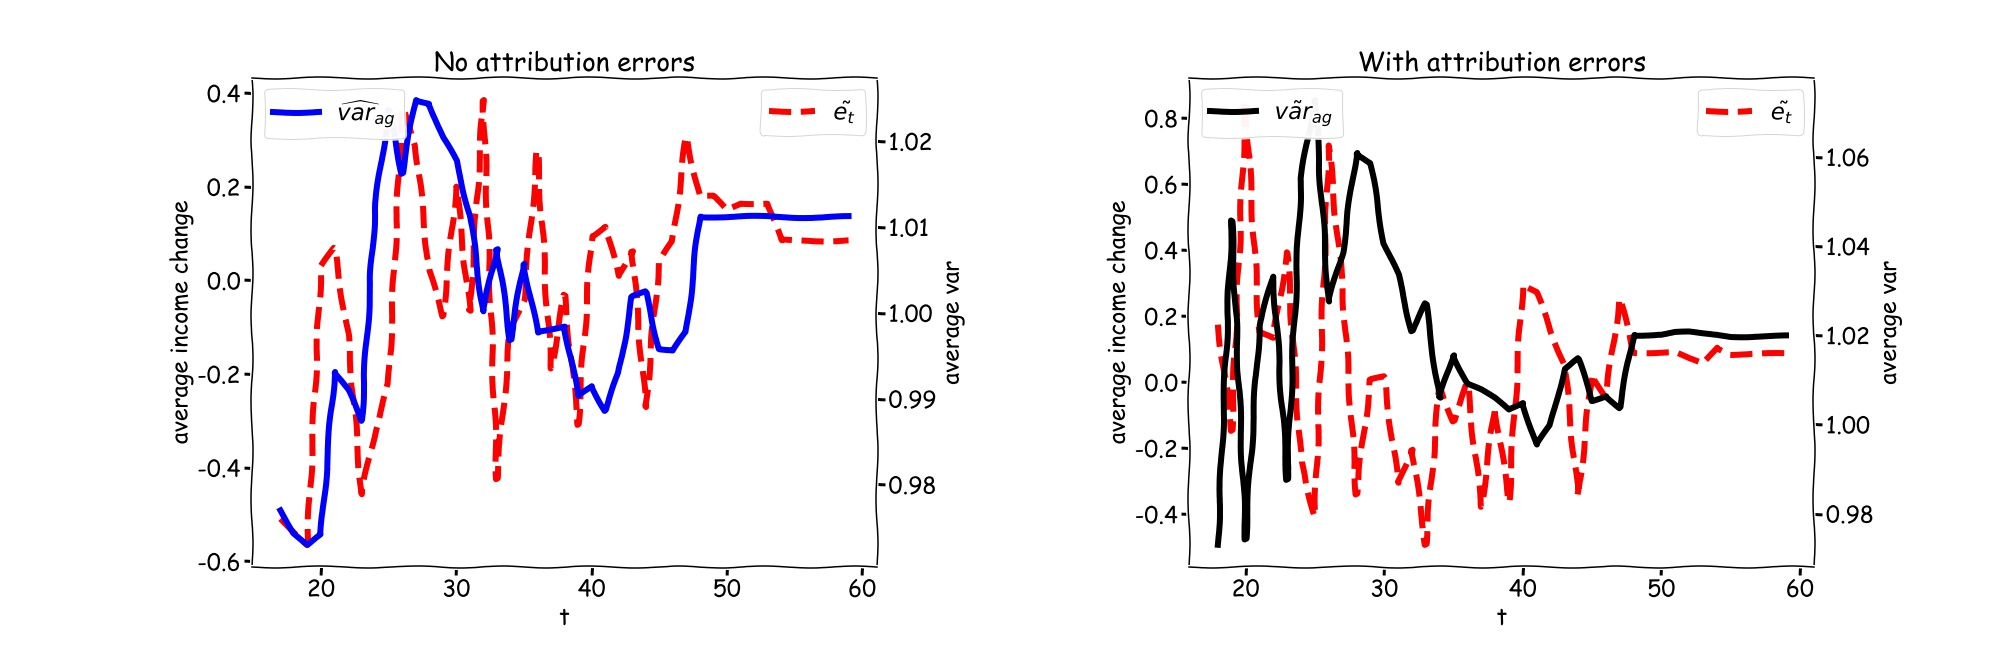
\includegraphics[width=\textwidth]{figures/var_recent_change_sim.jpg}
%	\end{figure}
%	\begin{figure}
%		\centering 
%		\label{var_experience_var}
%		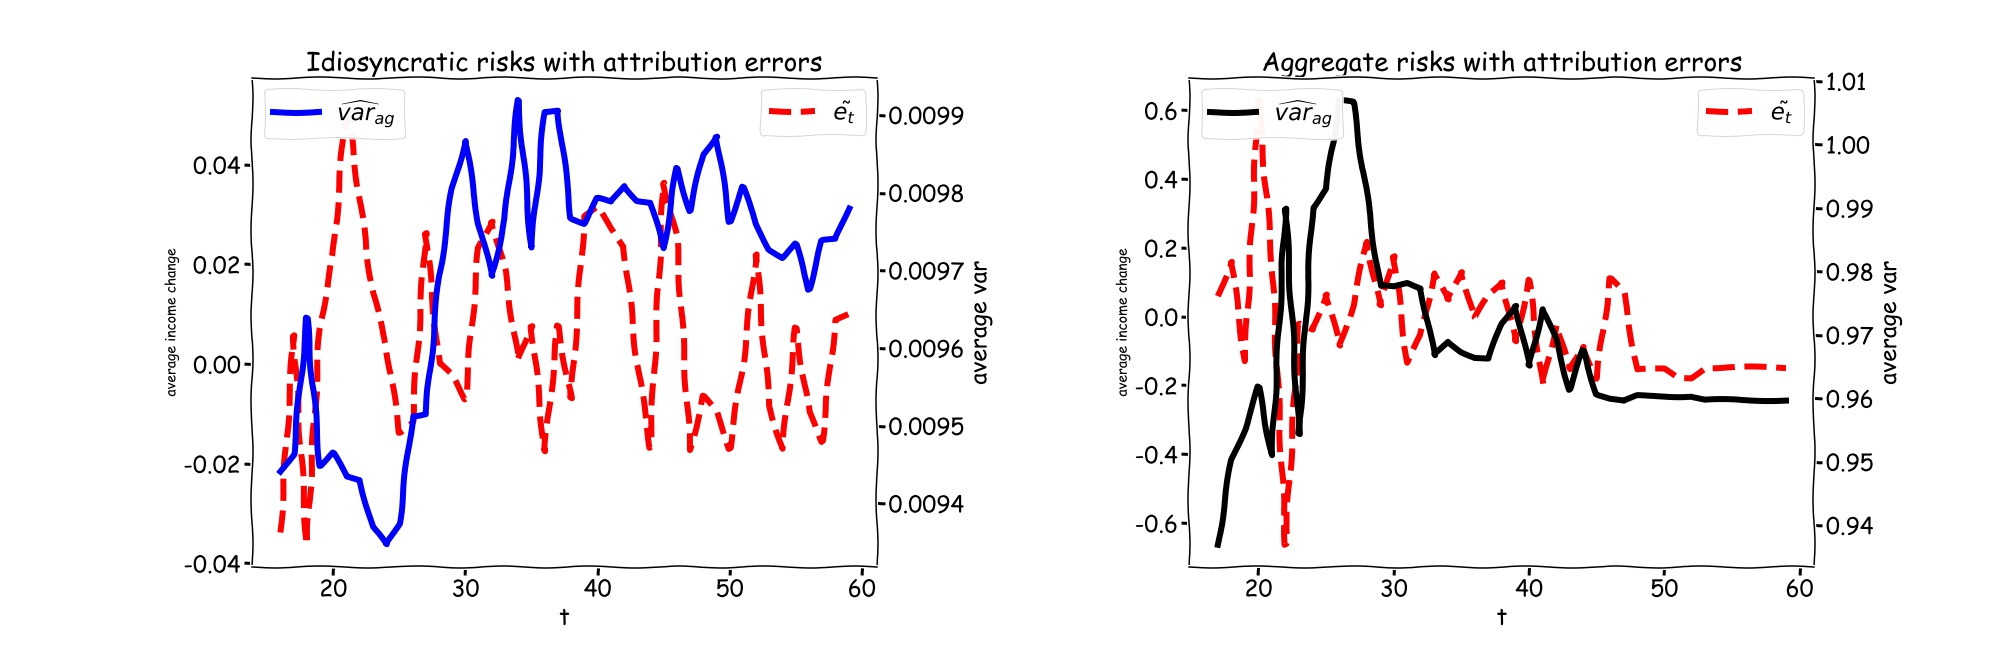
\includegraphics[width=\textwidth]{figures/var_recent_change_sim2.jpg}
%	\end{figure}
%\end{frame}


%\begin{frame}{Prediction 4. perceived risk declines over age}
%	\begin{figure}
%		\centering 
%		\label{var_experience_var}
%		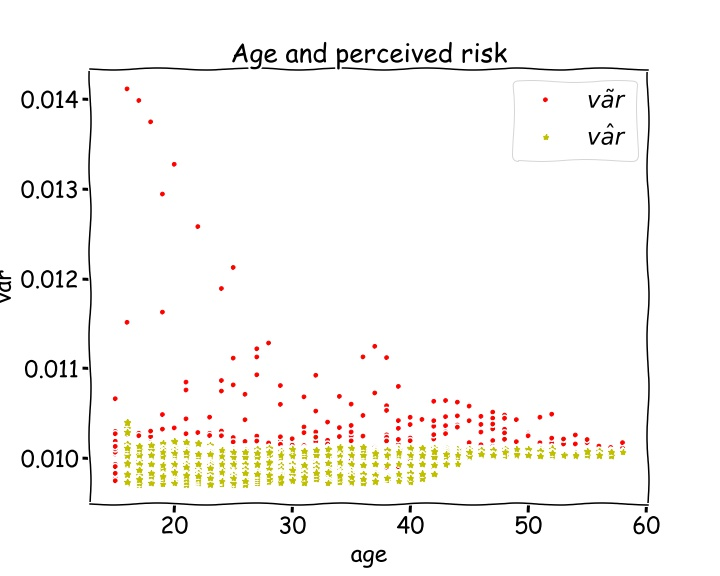
\includegraphics[width=0.7\textwidth]{figures/var_age_sim.jpg}
%	\end{figure}
%\end{frame}


%\begin{frame}{Prediction 3. skewed U-shaped income profile}
%	\begin{eqnarray}
%		\begin{split}
%			\tilde {Var}_{i,t}(\Delta y_{i,t+1})  = [(\sum^{t-c}_{k=0}\sum^{n}_{j=1}y^2_{j,t-k-1})^{-1}(1+\tilde\delta_{i,t}(n-1))y^2_{i,t} + 1] s^2_{i,t} 
%		\end{split}
%	\end{eqnarray}
%		\begin{figure}
%		\centering 
%		\label{var_experience_var}
%		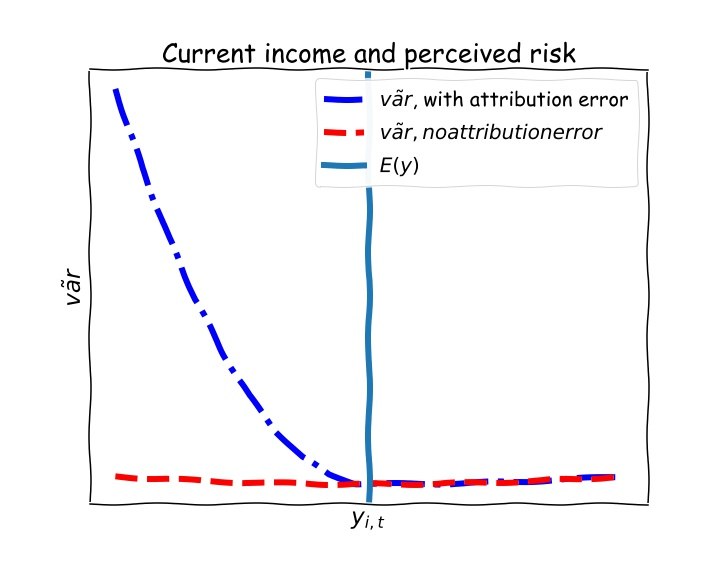
\includegraphics[width=0.6\textwidth, height = 0.6\textheight]{figures/var_recent.jpg}
%	\end{figure}
%\end{frame}



%\subsection{Simulation}	


%\begin{frame}{Simulated income profile}
%	\begin{figure}
%		\centering 
%		\label{var_experience_var}
%		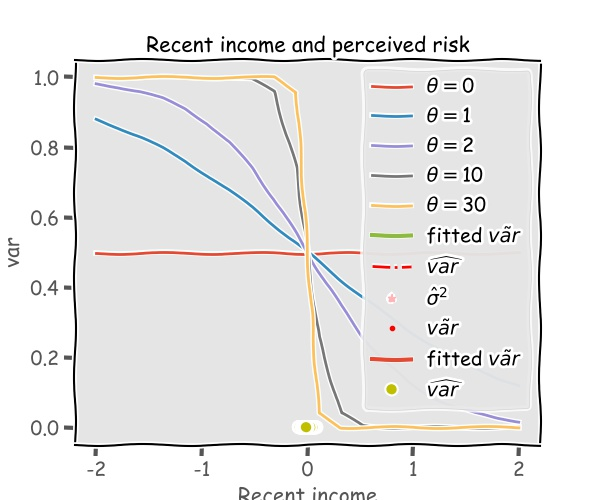
\includegraphics[width=0.7\textwidth]{figures/var_recent_sim.jpg}
%	\end{figure}
%\end{frame}



%\begin{frame}{Robustness}
%	\begin{itemize}
%		\item Permanent and transitory income risk 
%		\item Serial correlation 
%		\item Time-varying income risks 
%		\item More regressors 
%	\end{itemize}
%\end{frame}




\section{Summary}

\begin{frame}{Taking stock}

		\begin{itemize}
			\item People do have some clues 
		\begin{itemize}
			\item  consistent with inter-group differences in income volatility
			\item other covariates 
			\begin{itemize}
				\item $\downarrow$ with education, household income, being a male
				\item $\uparrow$  with numeracy score, self-employed job, perceived individual UE risks, and aggregate UE expectations 
			\end{itemize}
		\end{itemize}
			\item But huge amount of heterogeneity remains
			\begin{itemize}
				\item including all above: $R^2 =0.10$
				\item individual fixed effects only: $R^2=0.71$
			\end{itemize}
		\item Possible explantions
			\begin{itemize}
				\item state dependence: aggregate economy conditions matter  
				\item past dependence: experiences matters \cite{kuchler2019personal}
				\item imperfect understanding of the nature of the risks 
				\item intrinsic heterogeneity: some are more uncertain than the other \cite{ben2018expectations} 
			\end{itemize}
		\end{itemize} 
\end{frame}


\begin{frame}{A simple model of risk perception}
	\label{model}
	\begin{itemize}
		\item Under FIRE 
		\begin{equation*}
			\begin{split}
				&{ Var}^*_{i,c,t}(\Delta y_{i,c,t}) =  \sigma^2_{\psi,c} + \sigma^2_{\epsilon,c} 
			\end{split}
		\end{equation*}
		\item  Under imperfect understanding
		\begin{itemize}
			\item $\phi$ and $\sigma^2_{\epsilon,c}$ are not perfectly known 
			\item all realized shocks are perfectly observed  
		\end{itemize}
	\end{itemize}
	\begin{equation*}
		\begin{split}
			& \widetilde{ Var}_{i,c,t}(\Delta y_{i,c,t+1}) =  \sigma^2_{\psi,c} + \tilde \sigma^2_{\epsilon,c,t} \\
			&\textcolor{blue}{\text{Experience-dependence: }}	\tilde \sigma^2_{\epsilon,c,t} =  \frac{\overbrace{Var_{i,c,t}(\eta_{i,c,t})}^{\text{experienced volatility}} }{1+\tilde \phi^2_{i,c,t}} \\
			&\textcolor{blue}{\text{State-dependence: }}		\tilde \phi_{i,c,t} =  \delta(\epsilon_{i,c,t})  
		\end{split}
	\end{equation*}
\end{frame}

\begin{frame}{Implications for consumption/saving}
	\begin{itemize}
		\item \textcolor{blue}{heterogenous risk perceptions} within groups: 
		\begin{itemize}
			\item heterogeneity in PR $\rightarrow$ hetergeneity in saving/wealth
		\end{itemize}
		\item \textcolor{blue}{countercylical risks}: idiosyncratic risks are negatively correlated with aggregate state of the economy 
		\begin{itemize}
			\item stochastic risks induce more precautionary savings in aggregate \cite{caballero1990consumption}, \cite{meghir2004income}
			\item aggregate impacts of shocks to income risks \cite{bayer2019precautionary}
		\end{itemize}
		%\item \textcolor{blue}{non-log-normality}: allow for tail risks
	%	\begin{itemize}
	%		\item additional precautionary saving motives \cite{caballero1990consumption}
	%	\end{itemize}
	\end{itemize}
\end{frame}


%%%%%%%%%%%%%%%%%%%%%%%%%%

%% sumplement 

\section*{Appendix}



\begin{frame}{Within-group dispersion in nominal PR}
	\label{appendix:incstd}
	\begin{figure}
		\centering
		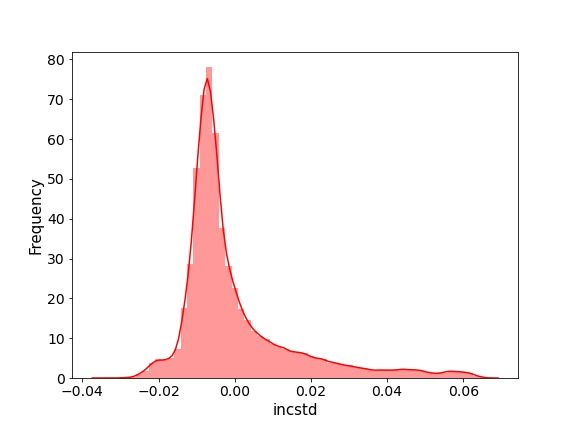
\includegraphics[width=0.65\textwidth]{figures/hist_incstd.jpg}
	\end{figure}
	\begin{itemize}
		\item  residuals controling for observables/time fixed effects
		\item average PR:  $2.1\%$ in std; 10/90 IQR: $3.2\%$ in std \quad \hyperlink{rincstd_hist}{\beamerbutton{Back}}    
		% \item just a lower bound: before adjustment of unemployment risk 
	\end{itemize}
\end{frame}


\begin{frame}{Within-group dispersion in PR skewness}
	\label{appendix:incskew}
	\begin{figure}
		\centering
		%			\begin{subfigure}[b]{0.45\textwidth}
		%			\centering
		%			\caption{income risks (nominal)}
		%		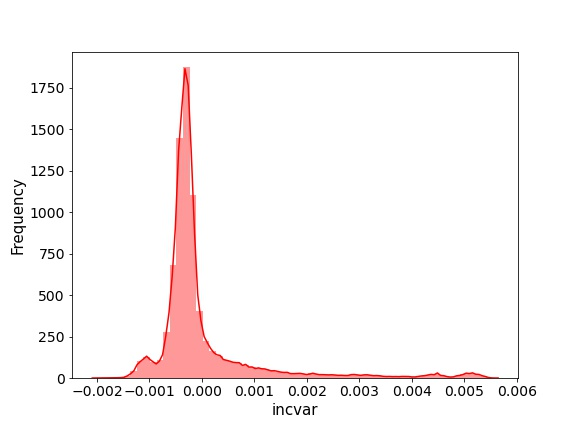
\includegraphics[width=\textwidth]{figures/hist_incvar.jpg}
		%		\end{subfigure}
		%	\begin{subfigure}[b]{0.45\textwidth}
		%		\centering
		%		\caption{income risks}
		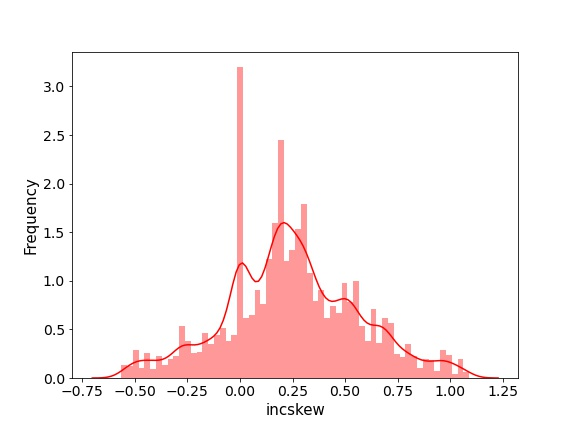
\includegraphics[width=0.65\textwidth]{figures/hist_incskew.jpg}
		%	\end{subfigure}
	\end{figure}
	\begin{itemize}
		\item  residuals controling for observables/time fixed effects
		%\item average PR:  $3.5\%$ in std; 10/90 IQR: $6.4\%$ in std 
			\quad \hyperlink{rincstd_hist}{\beamerbutton{Back}}    
		% \item just a lower bound: before adjustment of unemployment risk 
	\end{itemize}
\end{frame}

\begin{frame}{Appendix: PR by age/gender/education}
	\begin{figure}[ht]
		%\caption{Perceived Risk} 
		\label{appendix:age_gender_educ_compare_figure}
		\centering
		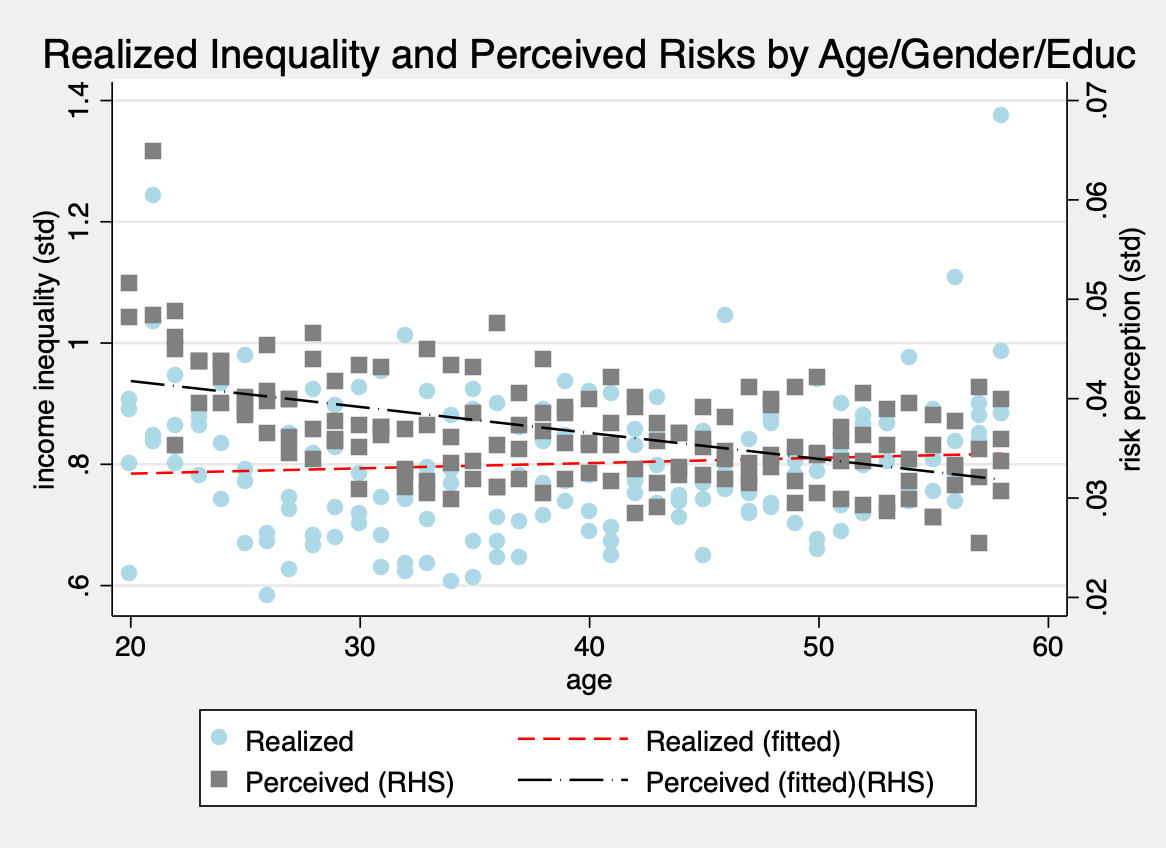
\includegraphics[width=0.7\textwidth]{figures/real_log_wage_shk_by_age_edu_gender_compare.png}
	\end{figure}
	\begin{itemize}
		\item age /gender/education  \quad  \hyperlink{age_compare}{\beamerbutton{Back}} 
		%	\item in line with existing findings, for instance  
		%	\cite{bloom2018great}. 
	\end{itemize}
\end{frame}

\begin{frame}{Appendix: PR by age}
	\begin{figure}[ht]
		%\caption{Perceived Risk} 
		\label{appendix:age_compare_figure}
		\centering
		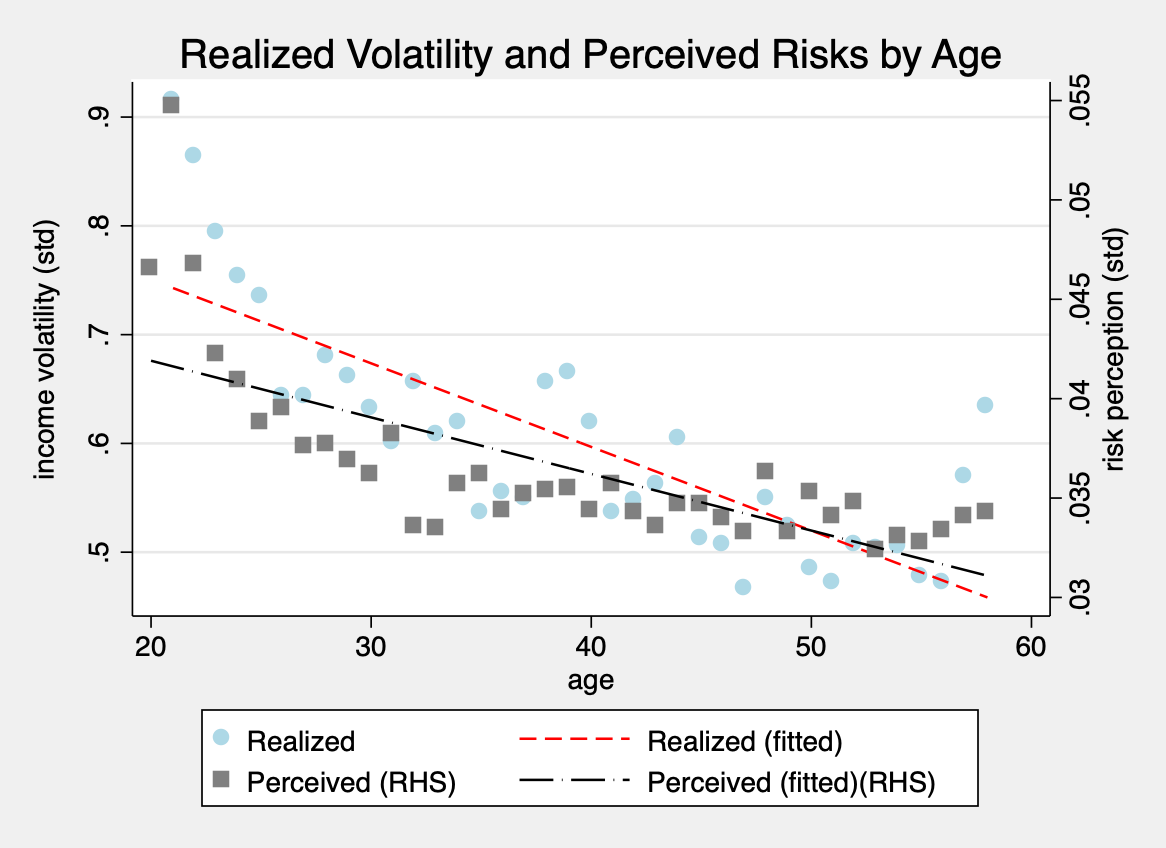
\includegraphics[width=0.7\textwidth]{figures/real_log_wage_shk_gr_by_age_compare.png}
	\end{figure}
	\begin{itemize}
		\item e.g. a 35-year old   \quad  \hyperlink{age_compare}{\beamerbutton{Back}} 
		%	\item in line with existing findings, for instance  
		%	\cite{bloom2018great}. 
	\end{itemize}
\end{frame}


\begin{frame}{Appendix: PR by age/education}
	\begin{figure}[ht]
		%\caption{Perceived Risk} 
		\label{appendix:age_educ_compare_figure}
		\centering
		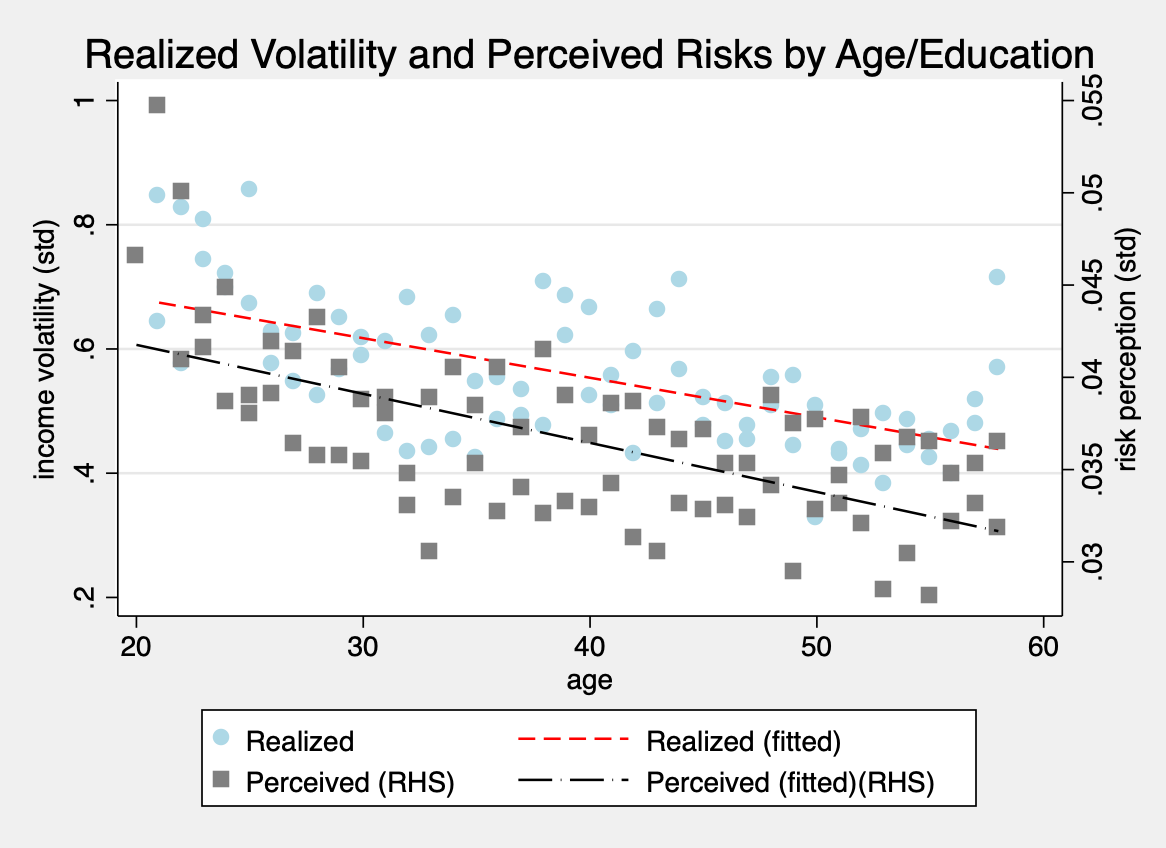
\includegraphics[width=0.7\textwidth]{figures/real_log_wage_shk_gr_by_age_edu_compare.png}
	\end{figure}
	\begin{itemize}
		\item e.g. a 35-year old high school graduate \quad  \hyperlink{age_compare}{\beamerbutton{Back}} 
		%	\item in line with existing findings, for instance  
		%	\cite{bloom2018great}. 
	\end{itemize}
\end{frame}



\begin{frame}{Appendix: PR by cohort/education/gender}
	\label{cohort_compare}
	\begin{figure}[ht]
		\label{appendix: compare_by_cohort}
		\centering
		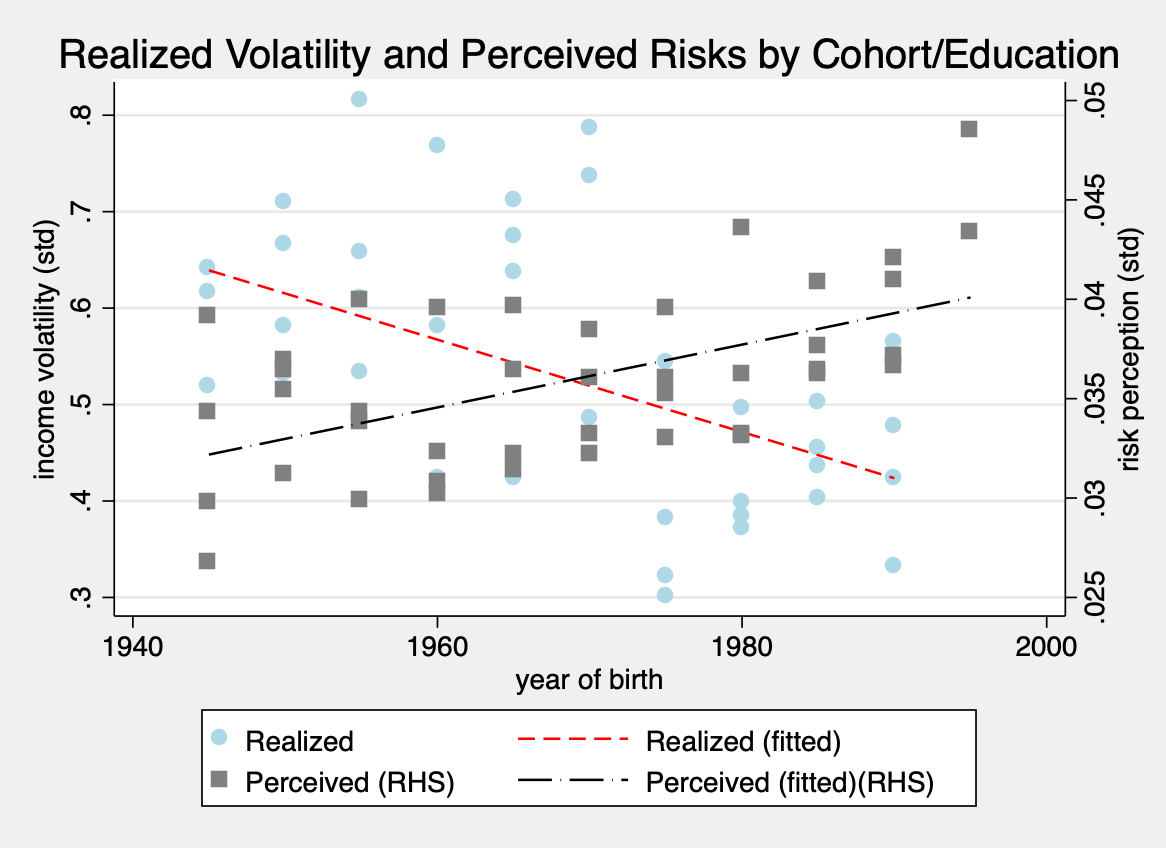
\includegraphics[width=0.6\textwidth]{figures/real_log_wage_shk_gr_by_byear_5yr_edu_gender_compare.png}
	\end{figure}
	\begin{itemize}
		\item e.g. a male higher school graduate born between 1990-1995 \quad \hyperlink{appendix:cohort_compare_figure}{\beamerbutton{inequality}}   
		\quad \hyperlink{appendix1:cohort_edu_compare_figure}{\beamerbutton{inequality by 5-year/education}}   
		\quad \hyperlink{appendix2:cohort_edu_compare_figure}{\beamerbutton{5-year/education}}     \quad  \hyperlink{age_compare}{\beamerbutton{Back}} 
		\item declining income volatlity between 1978-2013 \cite{sabelhaus2010great}, \cite{bloom2018great} 
	\end{itemize}
\end{frame}

\begin{frame}{Appendix: PR by cohort}
	\begin{figure}[ht]
		%\caption{Perceived Risk} 
		\label{appendix:cohort_compare_figure}
		\centering
		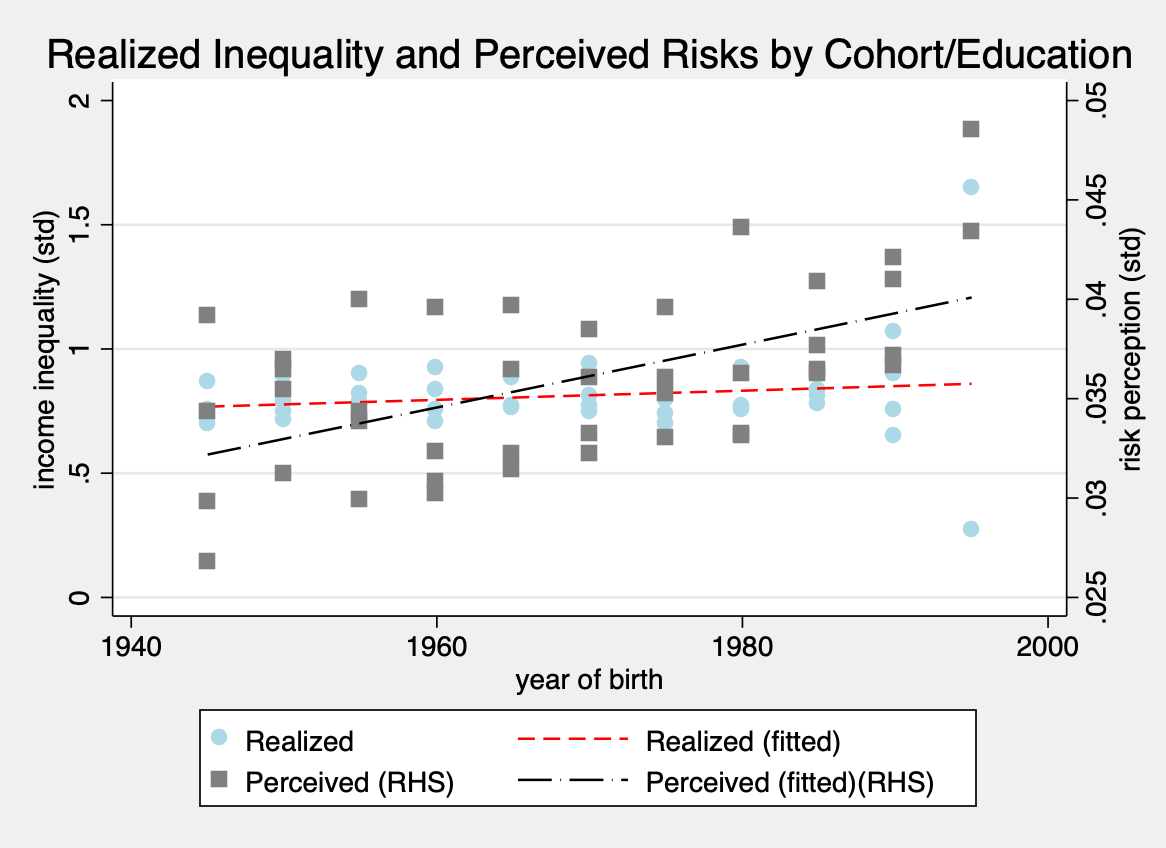
\includegraphics[width=0.7\textwidth]{figures/real_log_wage_shk_by_byear_5yr_edu_gender_compare.png}
	\end{figure}
	\begin{itemize}
		\item e.g. a female college graduate born between 1970-1975   \quad  \hyperlink{cohort_compare}{\beamerbutton{Back}} 
		%	\item in line with existing findings, for instance  
		%	\cite{bloom2018great}. 
	\end{itemize}
\end{frame}


\begin{frame}{Appendix: PR by cohort/education}
	\begin{figure}[ht]
		%\caption{Perceived Risk} 
		\label{appendix1:cohort_edu_compare_figure}
		\centering
		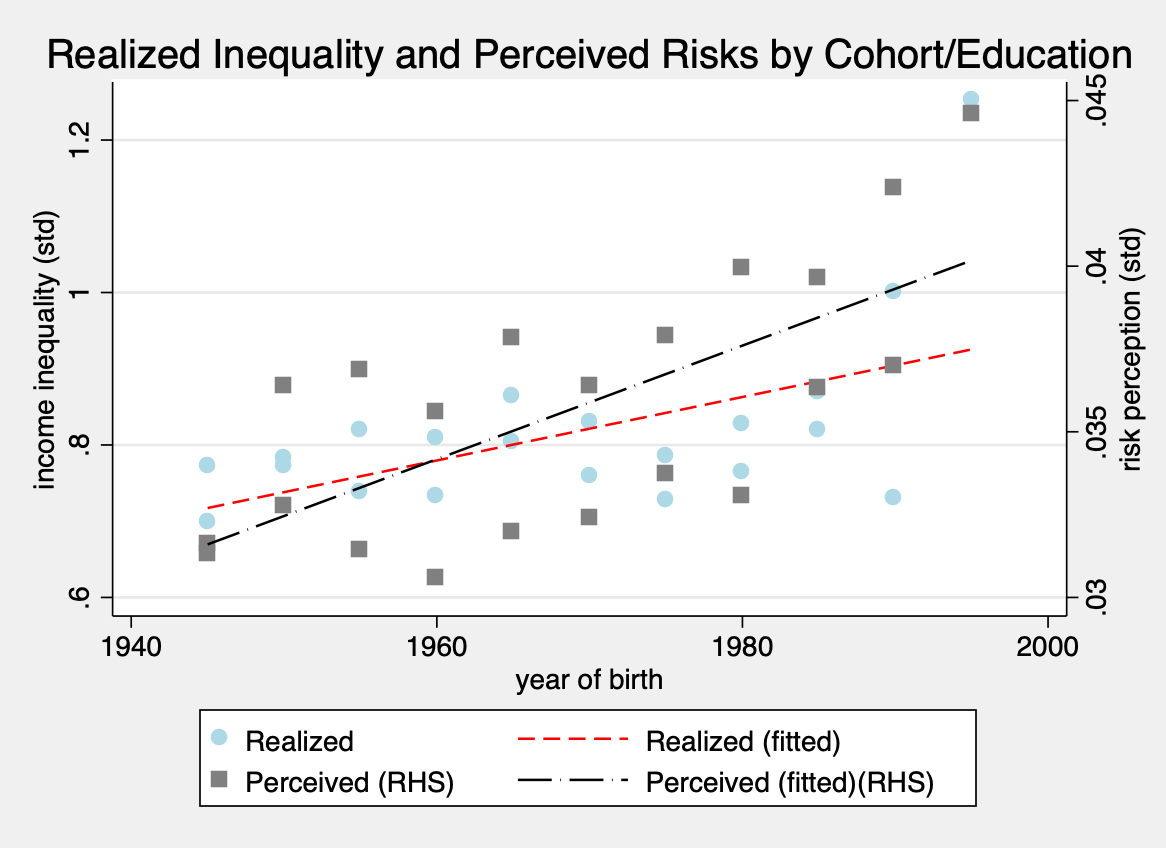
\includegraphics[width=0.7\textwidth]{figures/real_log_wage_shk_by_byear_5yr_edu_compare.png}
	\end{figure}
	\begin{itemize}
		\item e.g. a high school graduate born between 1985-1990  \quad  \hyperlink{cohort_compare}{\beamerbutton{Back}} 
		%	\item in line with existing findings, for instance  
		%	\cite{bloom2018great}. 
	\end{itemize}
\end{frame}


\begin{frame}{Appendix: PR by cohort/education}
	\begin{figure}[ht]
		%\caption{Perceived Risk} 
		\label{appendix2:cohort_edu_compare_figure}
		\centering
		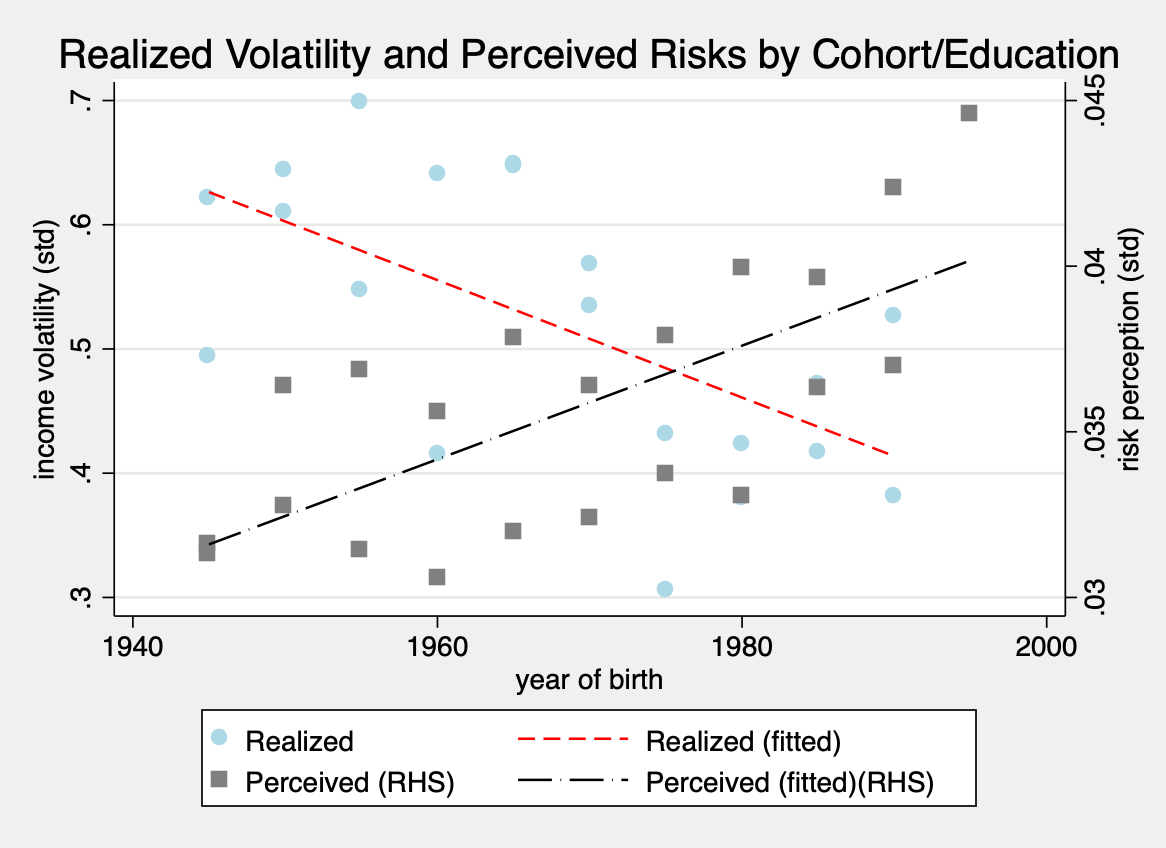
\includegraphics[width=0.7\textwidth]{figures/real_log_wage_shk_gr_by_byear_5yr_edu_compare.png}
	\end{figure}
	\begin{itemize}
		\item a college graduate born between 1985-1990  \quad  \hyperlink{cohort_compare}{\beamerbutton{Back}} 
		%	\item in line with existing findings, for instance  
		%	\cite{bloom2018great}. 
	\end{itemize}
\end{frame}



\begin{frame}{Appendix: expected income growth and recent (past) wage growth}
	\label{appendix:tsMean3mvrexp_he}
	\begin{itemize}
		\item $\overline{\text{exp}_{t}} $: average expected growth across individuals
		\item  quarterly growth in average hourly wage
	\end{itemize}
	\begin{figure}
		\centering
		\label{ts_exp}
		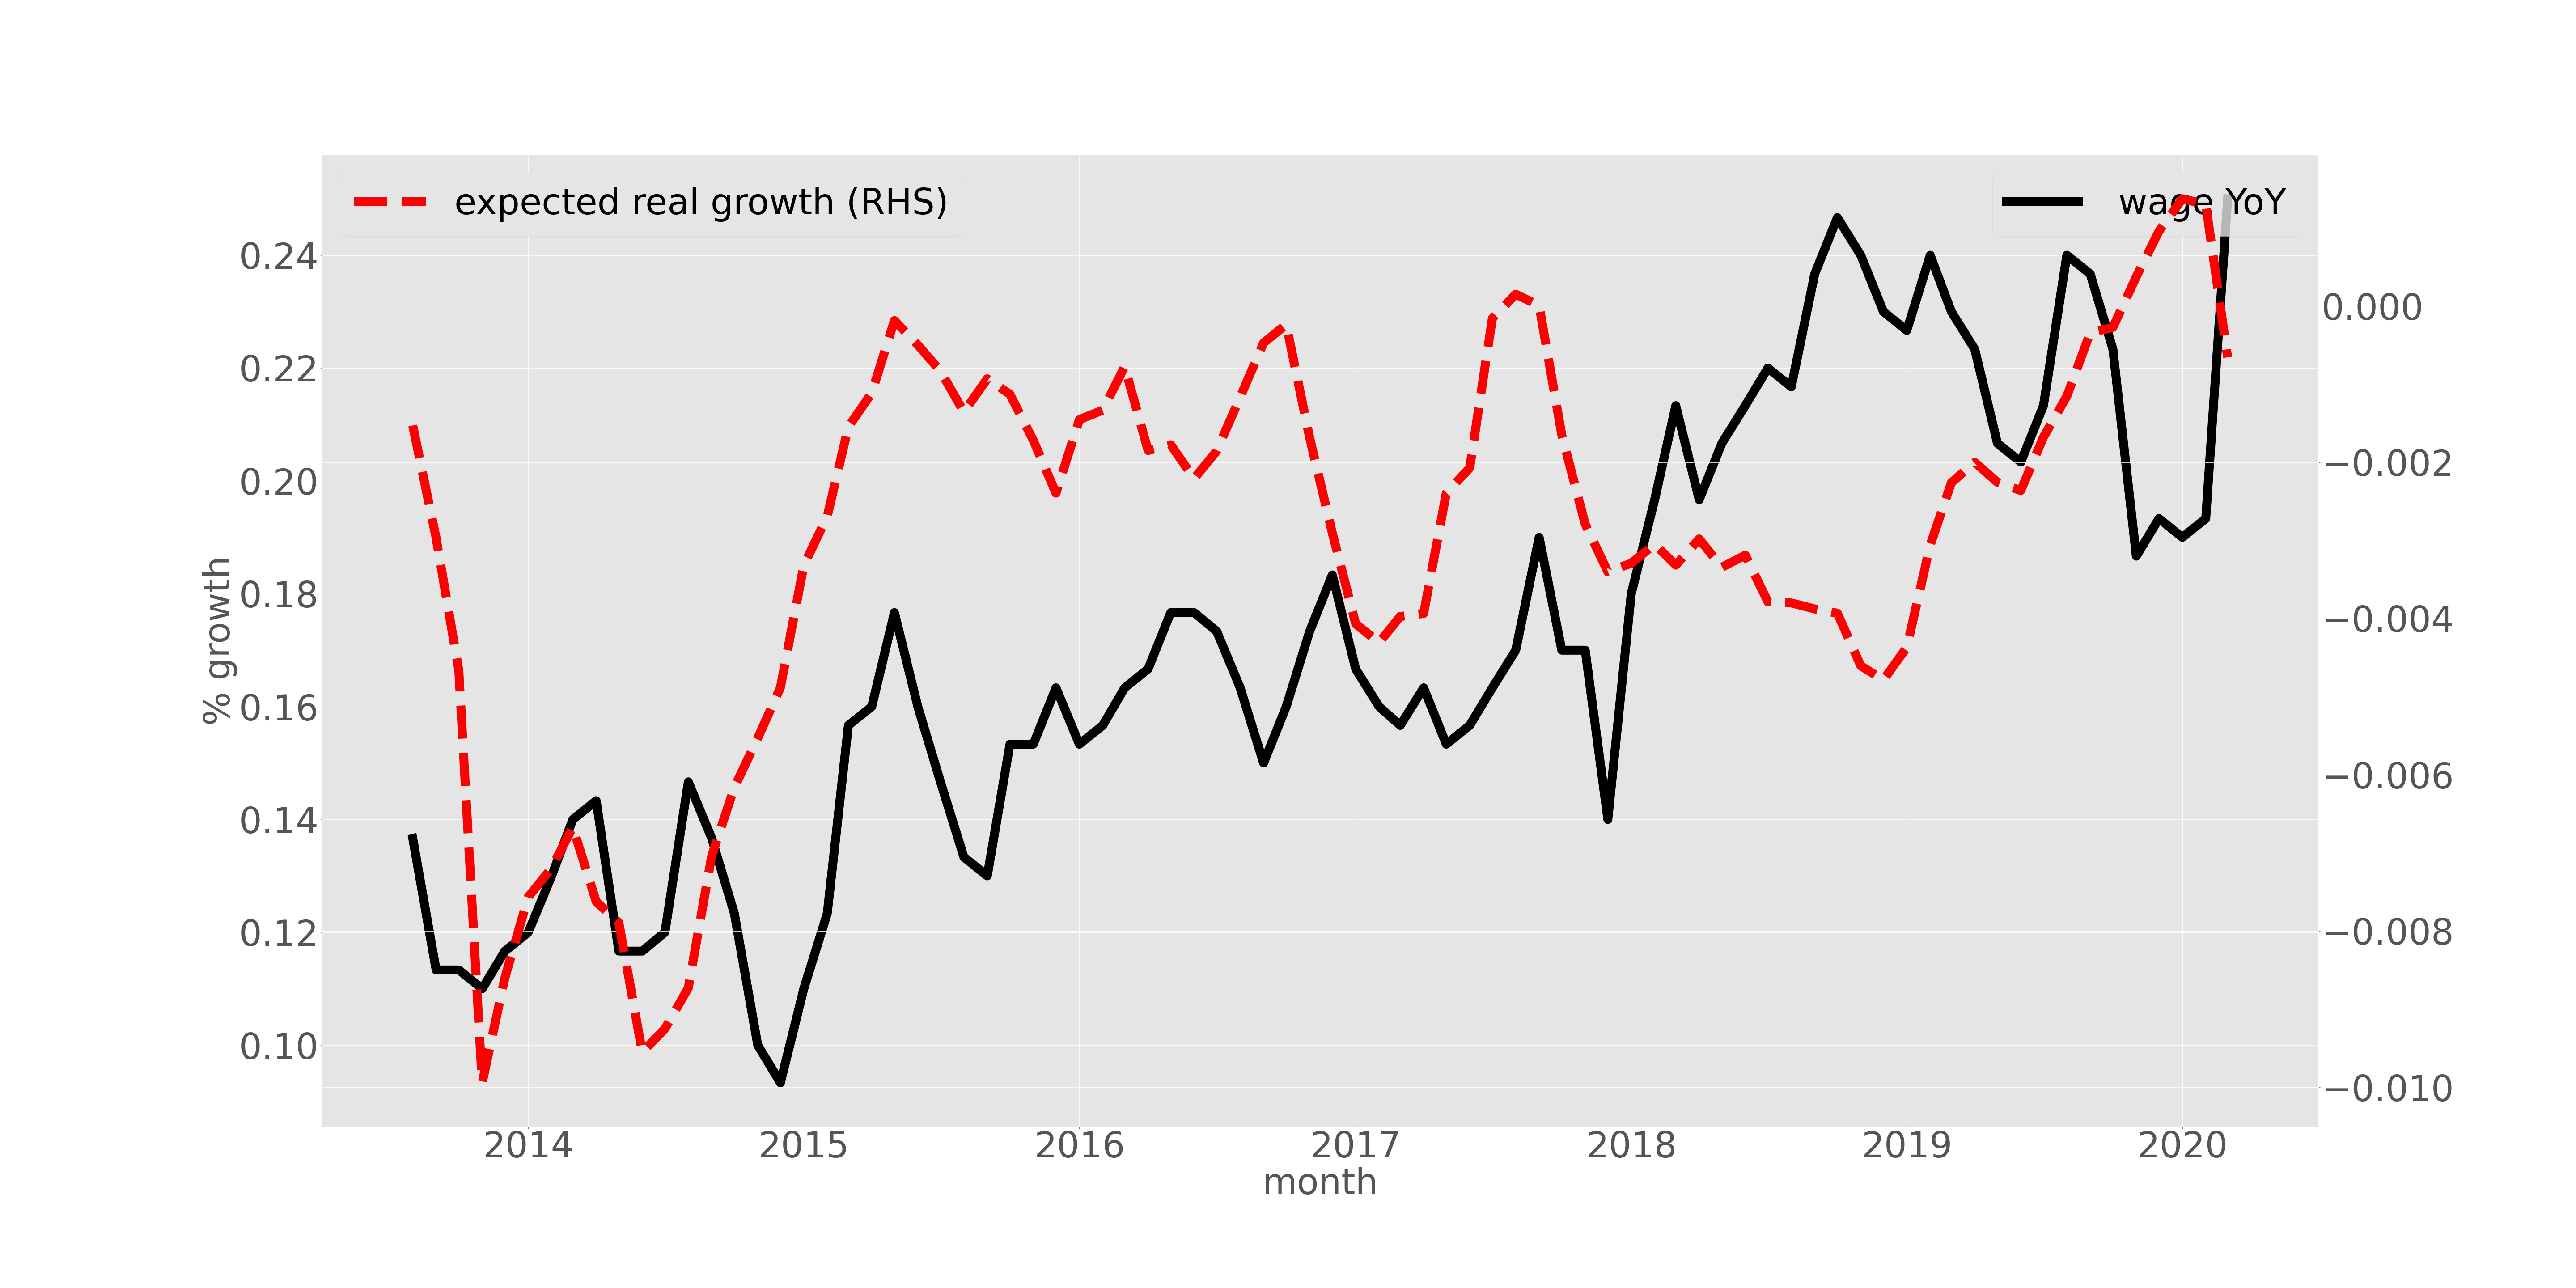
\includegraphics[width=0.9\textwidth]{figures/tsMean3mvrexp_he.jpg}
	\end{figure}
	\quad  \hyperlink{tsMean3mvrvar_he}{\beamerbutton{Back}} 
\end{frame}


\begin{frame}{Appendix: by \textbf{5-yr of birth/age}}
	\label{appendix:cohort_age_compare}
	\begin{figure}[ht]
		%\caption{Perceived Risk} 
		\centering
		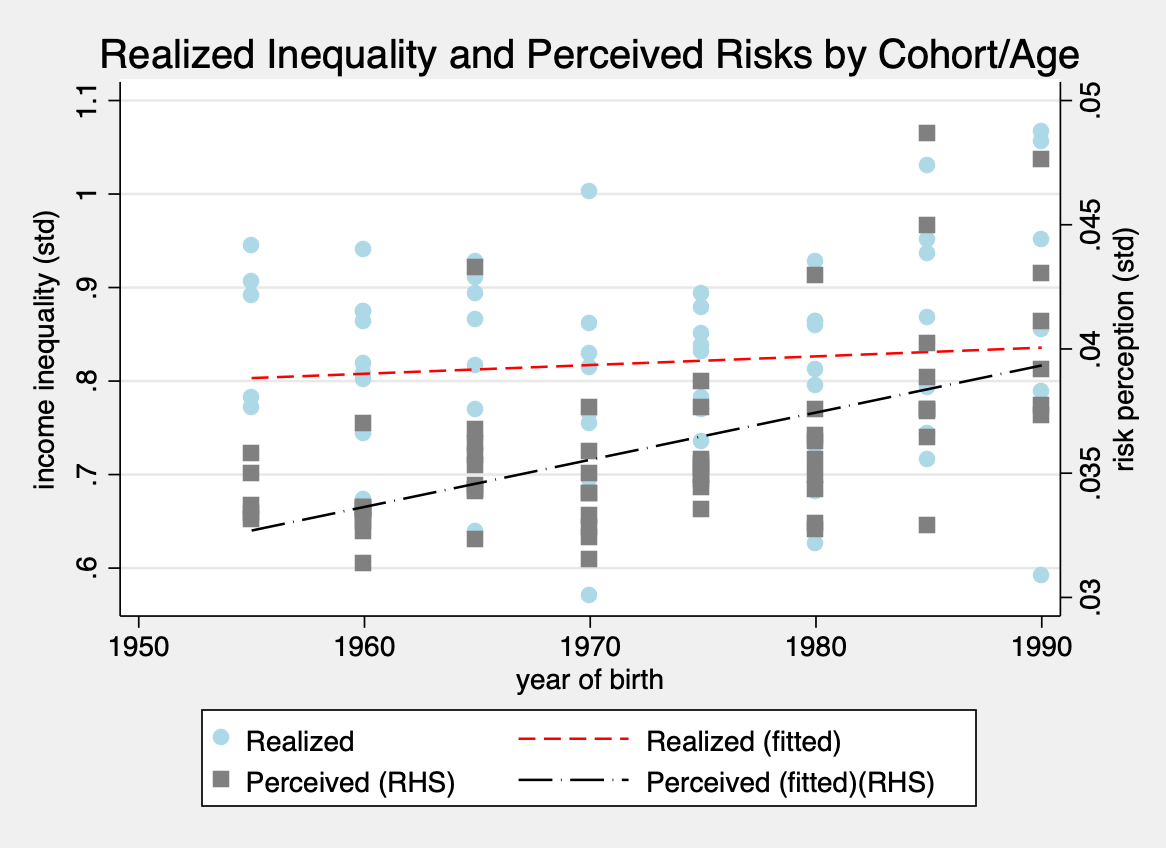
\includegraphics[width=0.65\textwidth]{figures/real_log_wage_shk_by_byear_age_compare.png}
		%	\begin{subfigure}[b]{0.46\textwidth}
		%			\caption{skewness}
		%			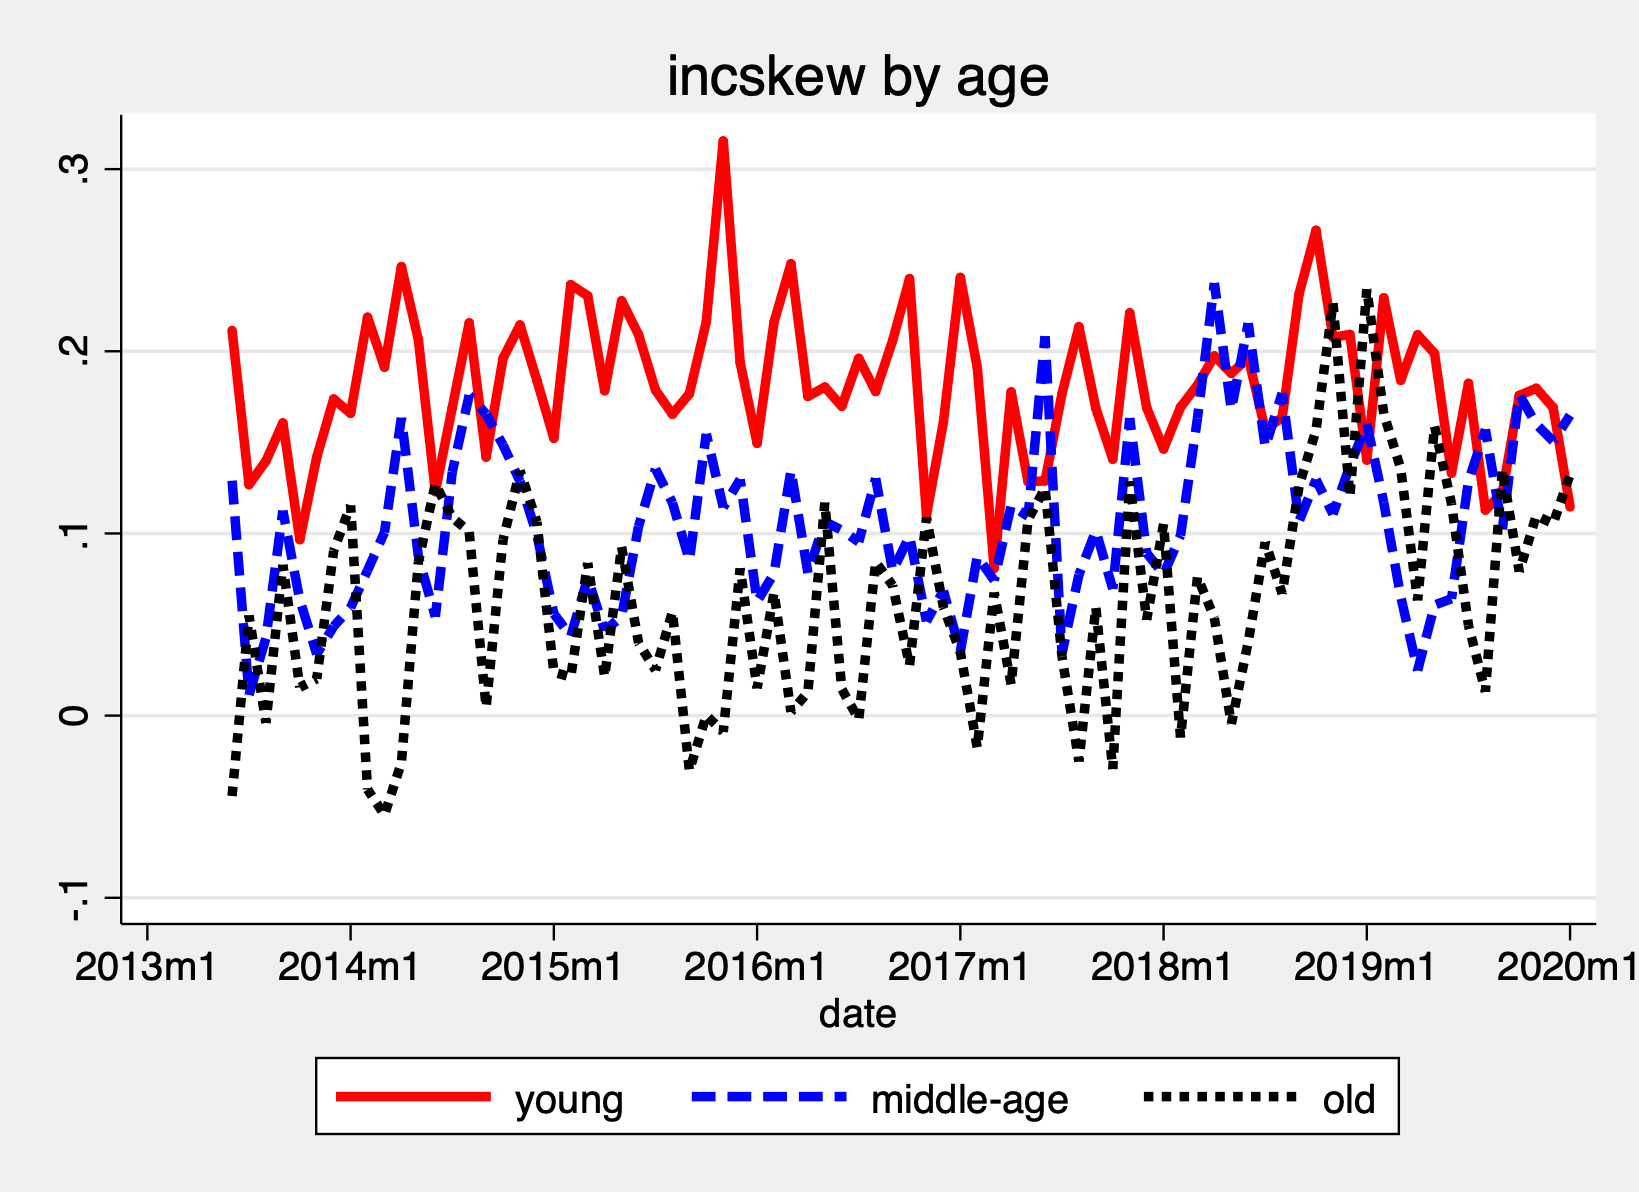
\includegraphics[width=\textwidth, height = 0.33\textheight]{figures/ts_incskew_age_g_mean.png}
		%	\end{subfigure}
	\end{figure}
	\begin{itemize}
		\item e.g. a 25-year old born between 1985-1990
		\item only possible for post-2013 sample 
		\quad \hyperlink{cohort_age_compare}{\beamerbutton{Back}}     
	\end{itemize}
\end{frame}

\begin{frame}{Appendix: permanent versus transitory risks}
	\label{appendix:cohort_age_component_compare}
	\begin{figure}[ht]
		%\caption{Perceived Risk} 
		\centering
		\begin{subfigure}[b]{0.44\textwidth}
			\caption{permanent}
			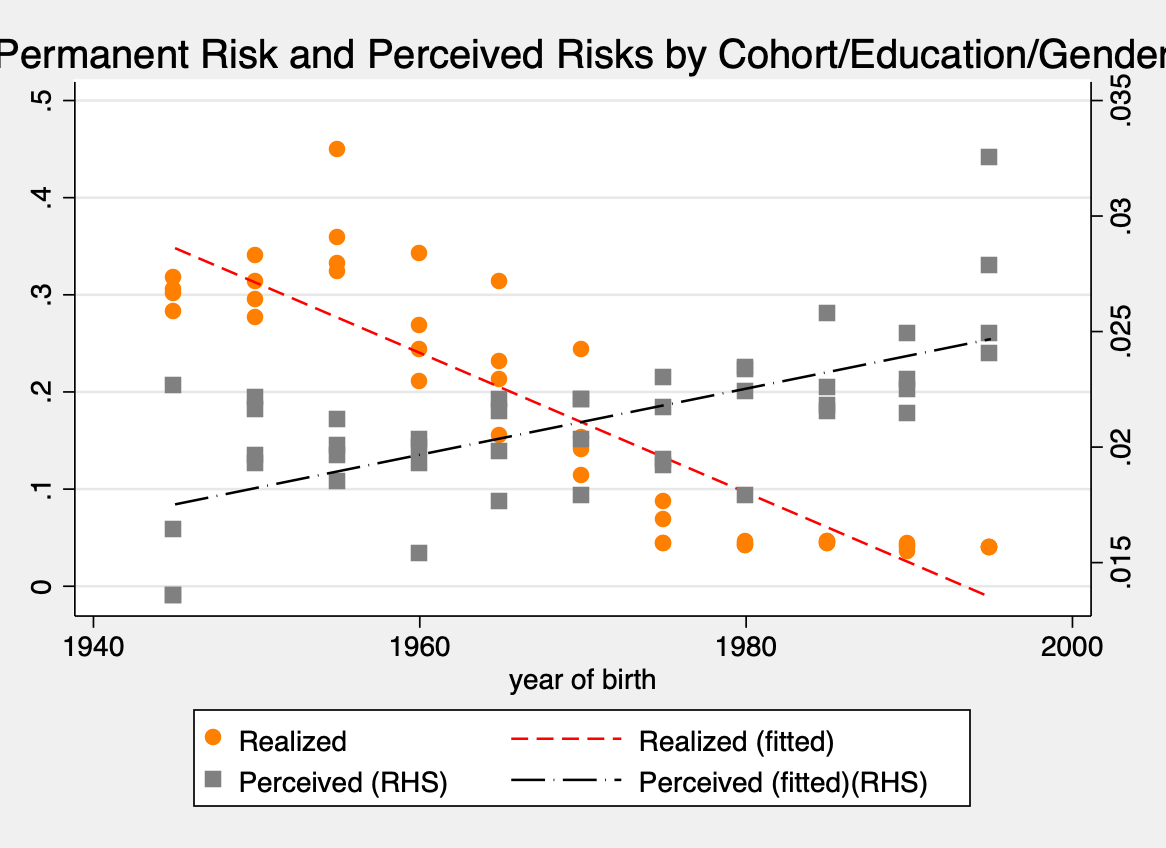
\includegraphics[width=\textwidth]{figures/log_wage_pshk_by_byear_5yr_edu_gender_compare.png}
		\end{subfigure}
		\begin{subfigure}[b]{0.44\textwidth}
			\caption{transitory}
			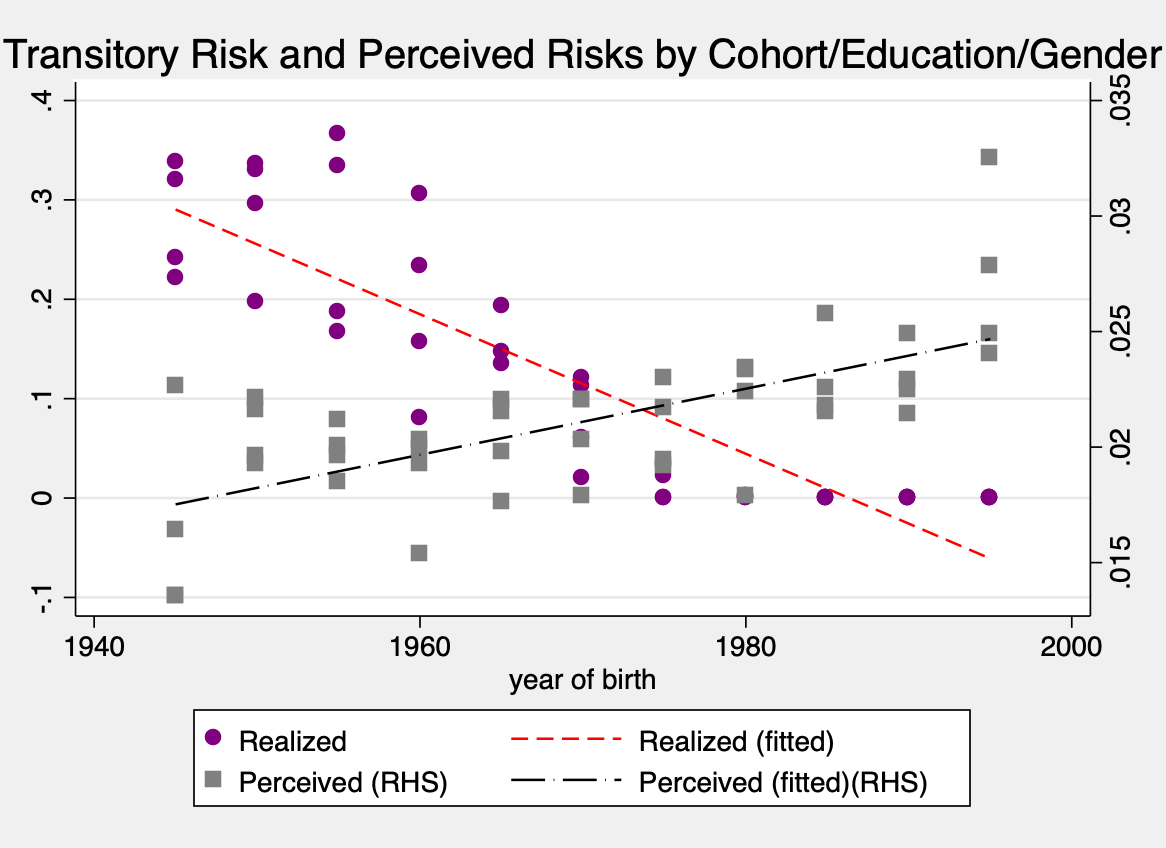
\includegraphics[width=\textwidth]{figures/log_wage_tshk_by_byear_5yr_edu_gender_compare.png}
		\end{subfigure} 
	\end{figure}
	\begin{itemize}
		\item e.g. a female high school graduate born between 1985-1990
		\quad  \hyperlink{cohort_age_component_compare}{\beamerbutton{Back}}  
	\end{itemize}
\end{frame}


\bibliographystyle{apalike}
\bibliography{PerceivedIncomeRisk}


\end{document}
